\setcounter{section}{2}
\setcounter{dang}{0}
\section{BIỂU THỨC TỌA ĐỘ CỦA CÁC PHÉP TOÁN VECTƠ}
\subsection{LÝ THUYẾT CẦN NHỚ}
\subsubsection{Biểu thức tọa độ của phép toán cộng, trừ, nhân một số thực với một vectơ}
Trong không gian $Oxyz$, cho hai véc-tơ $\vec{a} = (a_1;a_2;a_3)$, $\vec{b} = (b_1; b_2; b_3)$ và số $k$. Khi đó
\begin{listEX}[1]
	\item [\ding{172}] $\vec{a}+\vec{b}=(a_1+b_1;a_2+b_2;a_3+b_3)$;
	\item [\ding{173}] $\vec{a}-\vec{b}=(a_1-b_1;a_2-b_2;a_3-b_3)$;
	\item [\ding{174}] $k\vec{a} = (ka_1; ka_2; ka_3)$.
\end{listEX}
\begin{note}
	Cho hai véc-tơ $\vec{a}=(a_1;a_2;a_3)$, $\vec{b}=(b_1;b_2;b_3)$, $\vec{b}\ne \vec{0}$. Hai véc-tơ $\vec{a}$, $\vec{b}$ cùng phương khi và chỉ khi tồn tại một số thực $k$ sao cho $\heva{&a_1=k b_1\\& a_2= k b_2\\& a_3= k b_3.}$
\end{note}
\subsubsection{Biểu thức tọa độ của tích vô hướng hai vectơ}
Trong không gian $Oxyz$, tích vô hướng của hai véc-tơ $\vec{a} = (a_1;a_2;a_3)$ và $\vec{b} = (b_1; b_2; b_3)$ được xác định bởi công thức
\[\vec{a} \cdot \vec{b} = a_1b_1 + a_2b_2 + a_3b_3. \]
\begin{note}
	\begin{itemize}
		\item[\ding{172}] $\vec{a} \perp \vec{b} \Leftrightarrow a_1b_1 + a_2b_2 + a_3b_3 = 0$;
		\item[\ding{173}] $\left| \vec{a} \right| = \sqrt{a_1^2 + a_2^2 +a_3^2}$; \quad $AB=\sqrt{(x_B-x_A)^2+(y_B-y_A)^2+(z_B-z_A)^2}$.
		\item[\ding{174}] $\cos \left(\vec{a}; \vec{b}\right) = \dfrac{\vec{a}\cdot \vec{b}}{\left|\vec{a}\right| \cdot \left|\vec{b}\right|} = \dfrac{a_1b_1 + a_2b_2 + a_3b_3}{\sqrt{a_1^2 + a_2^2 +a_3^2} \cdot \sqrt{b_1^2 + b_2^2 +b_3^2}}$ (với $\vec{a},\vec{b} \ne \vec{0}$).
	\end{itemize}
\end{note}

\subsubsection{Biểu thức tọa độ của tích có hướng hai vectơ}
Cho hai véc-tơ $\vec{a}=(a_1;a_2;a_3)$ và $\vec{b}=(b_1;b_2;b_3)$ không cùng phương. Khi đó vec tơ $$\vec{w}=\bigg(a_2b_3-b_2a_3\,;\,a_3b_1-b_3a_1\,;\,a_1b_2-b_1a_2 \bigg)$$ vuông góc với cả hai véc tơ $\vec{a}$ và $\vec{b}$.
\begin{note}
	\begin{itemize}
		\item [\ding{172}] Véc tơ $\vec{w}$ xác định như trên còn gọi là \textbf{tích có hướng} của hai vectơ $\vec{a}$, $\vec{b}$, kí hiệu  $\vec{w}=\left[\vec{a},\vec{a}\right]$.
		\item [\ding{173}] Quy ước $\left|\begin{array}{l}
				      {a_1}\quad{a_2} \\
				      {b_1}\quad{b_2}
			      \end{array}\right|=a_1b_2-a_2b_1$ thì
		      $$\left[\vec a ,\vec b\right]=\left(\left|\begin{array}{l}
					      {a_2}\quad{a_3} \\
					      {b_2}\quad{b_3}
				      \end{array}\right|;\left|\begin{array}{l}
					      {a_3}\quad {a_1} \\
					      {b_3}\quad{b_1}
				      \end{array}\right|;\left|\begin{array}{l}
					      {a_1}\quad{a_2} \\
					      {b_1}\quad{b_2}
				      \end{array}\right|\right)$$
		\item [\ding{174}] $\vec{a}$ không cùng phương với $\vec{b}$ $\Leftrightarrow \left[\vec a ,\vec b\right] \ne \vec{0}$.
	\end{itemize}
\end{note}
\subsubsection{Ứng dụng của tích có hướng của hai véc-tơ}
	\begin{enumerate}
		\item Xét sự đồng phẳng của ba véc-tơ:
		\begin{itemize}
			\item Ba vectơ $\vec{a}$; $\vec{b}$; $\vec{c}$ đồng phẳng $\Leftrightarrow \left[ \vec{a},\vec{b} \right]\cdot \vec{c}=0$.
			\item Bốn điểm $A$, $B$, $C$, $D$ tạo thành tứ diện $\Leftrightarrow \left[ \vec{AB},\vec{AC} \right]\cdot \vec{AD}\ne 0$.
		\end{itemize}
		\item Diện tích hình bình hành: $S_{ABCD}=\left| \left[ \vec{AB},\vec{AD} \right] \right|$.
		\item Tính diện tích tam giác: $S_{\triangle ABC}=\dfrac{1}{2}\left| \left[ \vec{AB},\vec{AC} \right] \right|$.
		\item Tính thể tích hình hộp: $V_{ABCD.A'B'C'D'}=\left| \left[ \vec{AB},\vec{AC} \right]\cdot\vec{AA'} \right|$.
		\item Tính thể tích tứ diện: $V_{ABCD}=\dfrac{1}{6}\left| \left[ \vec{AB},\vec{AC} \right]\cdot \vec{AD} \right|$.
	\end{enumerate} 
\subsubsection{Biểu thức tọa độ trung điểm đoạn thẳng, trọng tâm tam giác}
\immini{Trong không gian $Oxyz$, tọa độ trung điểm và trong tâm được xác định như sau:
	\begin{itemize}
		\item [\ding{172}] Tọa độ trung điểm $M$ của đoạn thẳng $AB$ là
		      \[ M\left(\dfrac{x_A + x_B}{2}; \dfrac{y_A + y_B}{2}; \dfrac{z_A + z_B}{2} \right).\]
		\item [\ding{173}] Tọa độ trọng tâm $G$ của tam giác $ABC$ là
		      \[ G\left(\dfrac{x_A + x_B +x_C}{3}; \dfrac{y_A + y_B +y_C}{3}; \dfrac{z_A + z_B + z_C}{3} \right).\]
	\end{itemize}}
	{\begin{tikzpicture}[scale=0.8, font=\footnotesize, line join=round, line cap=round]
		\begin{scope}
			\foreach \x\y\t in {-2/-2/A, 0/0/B}
			\coordinate (\t) at (\x,\y);
			\coordinate (M) at ($(A)!0.5!(B)$);
			\foreach \a\b in {A/B}
			\draw[] (\a)--(\b);
			\foreach \t\g in {A/-90, B/40,M/1200}
			\draw[fill=black] (\t)circle(0.6pt) +(\g:8pt)node{$\t$};
		\end{scope}
		\begin{scope}[xshift=3cm]
			\foreach \x\y\t in {0/0/A, -2/-2/B, 2.5/-2/C}
			\coordinate (\t) at (\x,\y);
			\coordinate (M) at ($(A)!0.5!(B)$);
			\coordinate (N) at ($(A)!0.5!(C)$);
			\coordinate (K) at ($(C)!0.5!(B)$);
			\coordinate (G) at ($(A)!2/3!(K)$);
			\foreach \a\b in {A/B, B/C, A/C, A/K, M/C, B/N}
			\draw[] (\a)--(\b);
			\foreach \t\g in {A/90, B/-100, C/-80, M/120, N/40, K/-90,G/60}
			\draw[fill=black] (\t)circle(0.8pt) +(\g:10pt)node{$\t$};
		\end{scope}
	\end{tikzpicture}}
\subsection{PHÂN LOẠI VÀ PHƯƠNG PHÁP GIẢI TOÁN}
\begin{dang}{Tọa độ của các phép toán vec tơ, tọa độ điểm, độ dài đoạn thẳng}
\end{dang}
\BTTL
\begin{vd}
	Cho $\vec{a}=(-2 ; 3 ; 2), \vec{b}=(2 ; 1 ;-1), \vec{c}=(1 ; 2 ; 3)$. Tính tọa độ của mỗi vectơ sau:
	\begin{listEX}[3]
		\item $3 \vec{a}$;
		\item $2 \vec{a}-\vec{b}$;
		\item $\vec{a}+2 \vec{b}-\dfrac{3}{2} \vec{c}$.
	\end{listEX}
	\loigiai{
		Ta có
		\begin{listEX}
			\item $3 \vec{a}=(3 \cdot(-2) ; 3 \cdot 3 ; 3 \cdot 2)$. Vậy $3 \vec{a}=(-6 ; 9 ; 6)$.
			\item Ta có $2 \vec{a}=(-4 ; 6 ; 4)$ và $\vec{b}=(2 ; 1 ;-1)$.\\ Do đó, $2 \vec{a}-\vec{b}=(-4-2 ; 6-1 ; 4-(-1))$.\\
			Vậy $2 \vec{a}-\vec{b}=(-6 ; 5 ; 5)$.
			\item Do $\vec{a}=(-2 ; 3 ; 2)$ và $2 \vec{b}=(4 ; 2 ;-2)$ nên
			\[\vec{a}+2 \vec{b}=(2 ; 5 ; 0).\]
			Ngoài ra, vì $-\dfrac{3}{2} \vec{c}=\left(-\dfrac{3}{2} ;-3 ;-\dfrac{9}{2}\right)$ nên $\vec{a}+2 \vec{b}-\dfrac{3}{2} \vec{c}=\left(\dfrac{1}{2} ; 2 ;-\dfrac{9}{2}\right)$.
		\end{listEX}}
\end{vd}
\dongcham{8}
\begin{vd}
	Trong không gian $Oxyz$, cho các véc-tơ $\vec{u}=3\vec{i}-2\vec{j}+\vec{k}$, $\vec{v}=-\dfrac{3}{2}\vec{i}+\vec{j}-\dfrac{1}{2}\vec{k}$, $\vec{w}=6\vec{i}+m\vec{j}-n\vec{k}$.
	\begin{enumerate}
		\item Chứng minh $\vec{u}$ và $\vec{v}$ cùng phương.
		\item Tìm giá trị của $m$ và $n$ để véc-tơ $\vec{u}$ và $\vec{w}$ cùng phương.
	\end{enumerate}
	\loigiai{
		Ta có $\vec{u}=(3;-2;1)$, $\vec{v}=\left(-\dfrac{3}{2}; 1; -\dfrac{1}{2}\right)$, $\vec{w}=\left(6; m; -n\right)$.
		\begin{enumerate}
			\item Hai véc-tơ $\vec{u}$ và $\vec{v}$ cùng phương khi và chỉ khi
			      $$\vec{v}=k\vec{u}\Leftrightarrow{ \left\{\begin{aligned}& -\dfrac{3}{2}=3k\\&1=-2k\\&-\dfrac{1}{2}=k\end{aligned}\right.}\Leftrightarrow k=-\dfrac{1}{2}$$
			      Như vậy $ \vec{v}=-\dfrac{1}{2}\vec{u} $ nên hai véc-tơ $\vec{u}$ và $\vec{v}$ cùng phương.
			\item Hai véc-tơ $\vec{u}$ và $\vec{w}$ cùng phương khi và chỉ khi
			      $$\vec{w}=k\vec{u}\Leftrightarrow{ \left\{\begin{aligned}&6=3k\\&m=-2k\\&-n=k\end{aligned}\right.}\Leftrightarrow { \left\{\begin{aligned}&k=2\\&m=-4\\&n=-2\end{aligned}\right.}$$
			      Như vậy $ m=-4$ và $ n=-2 $ thì hai véc-tơ $\vec{u}$ và $\vec{w}$ cùng phương. Khi đó $\vec{w}=\left(6; -4; 2\right)$.
		\end{enumerate}
	}
\end{vd}
\dongcham{8}
\begin{vd}
	Trong không gian với hệ tọa độ $Oxyz$, cho ba điểm $A(3;-1;2)$, $B(1;2;3)$, $C(4;-2;1)$.
	\begin{tasks}
		\task Chứng minh ba điểm $A, B, C$ không thẳng hàng. Xác định tọa độ trọng tâm tam giác $ABC$.
		\task Tìm tọa độ điểm $D$ biết $ABCD$ là hình bình hành.
		\task Tìm tọa độ giao điểm $E$ của đường thẳng $BC$ với mặt phẳng tọa độ $\left(Oxz\right)$.
	\end{tasks}
	\loigiai{
		\begin{enumerate}
			\item Ta có $\vec{AB}=(-2;3;1)$, $\vec{AC}=(1;-1;-1)$.
			      Vì $\dfrac{-2}{1}\neq \dfrac{-3}{-1}$ nên hai véc-tơ $\vec{AB}$, $\vec{AC}$ không cùng phương.\\
			      Hay ba điểm $A$, $B$, $C$ không thẳng hàng. Suy ra, tọa độ trọng tâm là $G\left(\dfrac{8}{3};-\dfrac{1}{3};2 \right)$.
			\item
			      \immini{Tứ giác $ABCD$ là hình bình hành khi và chỉ khi
				      $$ \vec{DC}=\vec{AB}\Leftrightarrow{ \left\{\begin{aligned}&4-x_D=-2\\&-2-y_D=3\\&1-z_D=1\end{aligned}\right.}\Leftrightarrow {\left\{\begin{aligned}&x_D=6\\&y_D=-5\\&z_D=0\end{aligned}\right.}$$
				      Vậy $D(6;-5;0)$.
			      }{
				      \begin{tikzpicture}[scale=.8]
					      \tkzDefPoints{0/4/A,-2/0/B,3/0/C}
					      \coordinate (D) at ($(A)+(C)-(B)$);
					      \tkzDrawSegments(A,B B,C C,D D,A)
					      \tkzLabelPoints[left](A,B)
					      \tkzLabelPoints[right](C,D)
					      \tkzDrawPoints(A,B,C,D)
				      \end{tikzpicture}}
			\item Vì $E$ thuộc mặt phẳng $Oxz$ nên $E=(x;0;z)$.\\
			      Ta có $\vec{AE}=(x-3;1;z-2)$.\\
			      Mặt khác $A, B, E$ thẳng hàng nên hai véc-tơ $\vec{AB}$, $\vec{AE}$ cùng phương, do đó:
			      $$ \vec{AE}=k\vec{AB}\Leftrightarrow{ \left\{\begin{aligned}&x-3=-2k\\&1=3k\\&z-2=k\end{aligned}\right.}\Leftrightarrow {\left\{\begin{aligned}&x=\dfrac{7}{3}\\&k=\dfrac{1}{3}\\&z=\dfrac{7}{3}\end{aligned}\right.}$$
			      Vậy $E=\left(\dfrac{7}{3}; 0; \dfrac{7}{3}\right)$.
		\end{enumerate}
	}
\end{vd}
\dongcham{18}
\begin{vd}
	Trong không gian $Oxyz$, cho ba điểm $A(5;-3;0)$, $B(2;1;-1)$, $C(4;1;2)$.
	\begin{enumerate}
		\item Tìm tọa độ của vectơ $\vec{u}=2\vec{AB}+\vec{AC}-5\vec{BC}$.
		\item Tìm tọa độ điểm $N$ sao cho $2\vec{NA}=-\vec{NB}$.
	\end{enumerate}
	\loigiai{
		\begin{enumerate}
			\item Ta có $\heva{&A(5;-3;0)\\ &B(2;1;-1)\\&C(4;1;2)}\Rightarrow\heva{&\vec{AB}=(-3;4;-1)\\&\vec{AC}=(-1;4;2)\\&\vec{BC}=(2;0;3)}\Rightarrow\heva{&2\vec{AB}=(-6;8;-2)\\&\vec{AC}=(-1;4;2)\\&-5\vec{BC}=(-10;0;-15)}\Rightarrow \vec{u}=(-17;12;-15)$.
			\item Gọi $N(x;y;z)$, khi đó $\heva{&\vec{NA}=(5-x;-3-y;-z)\\&\vec{NB}=(2-x;1-y;-1-z)}$\\
			      $$2\vec{NA}=-\vec{NB}\Leftrightarrow \heva{&2(5-x)=-2+x\\&2(-3-y)=-1+y\\&-2z=1+z}\Leftrightarrow \heva{&x=4\\&y=-\dfrac{5}{3}\\&z=-\dfrac{1}{3}}\Rightarrow N\left(4;-\dfrac{5}{3};-\dfrac{1}{3}\right).$$
		\end{enumerate}
	}
\end{vd}
\dongcham{14}
\begin{vd}%[2H2H2-6]
	\immini{Một phòng học có thiết kế dạng hình hộp chữ nhật với chiều dài là $8$ m, chiều rộng là $6$ m và chiều cao là $3$ m. Một chiếc đèn được treo tại chính giữa trần nhà của phòng học. Xét hệ trục toạ độ $Oxyz$ có gốc $O$ trùng với một góc phòng và mặt phẳng $(Oxy)$ trùng với mặt sàn, đơn vị đo được lấy theo mét (\textit{Hình minh họa bên}). Hãy tìm toạ độ của điểm treo đèn.}{
		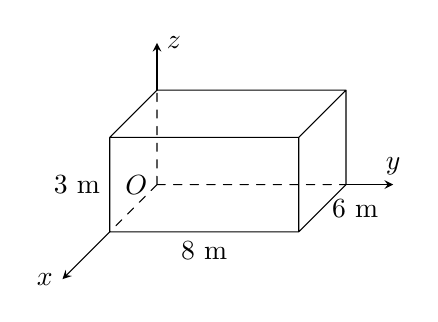
\begin{tikzpicture}[line cap=round,line join=round, >=stealth,scale=0.6]
			\path (0,0)coordinate[label=left:$O$](O) (-1,-1)coordinate(B) (4,0)coordinate(D) (3,-1)coordinate(C) (0,2)coordinate(O') (-1,1)coordinate(B') (3,1)coordinate(C') (4,2)coordinate(D') (0,3)coordinate[label=right:$z$](E) (5,0)coordinate[label=above:$y$](F) (-2,-2)coordinate[label=left:$x$](G) (-1,0)coordinate[label=left:$3$ m](H) (1,-1)coordinate[label=below:$8$ m](I)
			(3.5,-0.5)coordinate[label=right:$6$ m](K);
			\draw (B)--(B')--(C')--(C)--cycle (O')--(B') (O')--(D') (C')--(D') (D')--(D) (D)--(C);
			\draw[dashed] (O)--(B) (O)--(D) (O)--(O');
			\draw[->] (B)--(G);
			\draw[->] (O')--(E);
			\draw[->] (D)--(F);
		\end{tikzpicture}
	}
	\loigiai{
		\immini{Gọi các điểm $B(3;0;0)$, $C(3;6;0)$, $D(0;6;0)$ như hình vẽ.\\
			$N$ là trung điểm $OC$, $N'$ là hình chiếu của $N$ lên mặt phẳng trần nhà.\\
			Suy ra $N'$ là điểm treo đèn.\\
			Ta có $N$ có tọa độ là $\left(\dfrac{0+3}{2};\dfrac{0+6}{2};\dfrac{0+0}{2}\right)$, suy ra $N\left(\dfrac{3}{2};3;0\right)$.\\
			Suy ra $N'\left(\dfrac{3}{2};3;3\right)$.\\
			Vậy tọa độ của điểm treo đèn là $\left(\dfrac{3}{2};3;3\right)$.
		}
		{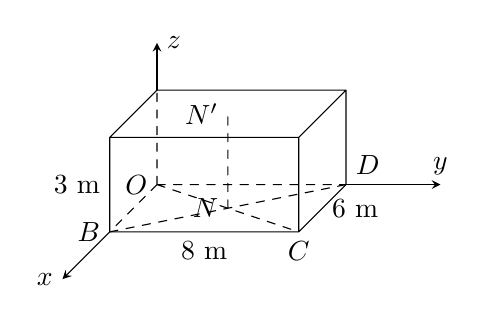
\begin{tikzpicture}[line cap=round,line join=round, >=stealth,scale=0.6]
				\path (0,0)coordinate[label=left:$O$](O) (-1,-1)coordinate[label=left:$B$](B) (4,0)coordinate[label=above right:$D$](D) (3,-1)coordinate[label=below:$C$](C) (0,2)coordinate(O') (-1,1)coordinate(B') (3,1)coordinate(C') (4,2)coordinate(D') (0,3)coordinate[label=right:$z$](E) (6,0)coordinate[label=above:$y$](F) (-2,-2)coordinate[label=left:$x$](G) (-1,0)coordinate[label=left:$3$ m](H) (1,-1)coordinate[label=below:$8$ m](I)
				(3.5,-0.5)coordinate[label=right:$6$ m](K);
				\coordinate[label=left:$N$] (N) at (intersection cs:first line={(O)--(C)}, second line={(B)--(D)});
				\coordinate[label=left:$N'$] (N') at (intersection cs:first line={(O')--(C')}, second line={(B')--(D')});
				\draw (B)--(B')--(C')--(C)--cycle (O')--(B') (O')--(D') (C')--(D') (D')--(D) (D)--(C);
				\draw[dashed] (O)--(B) (O)--(D) (O)--(O') (O)--(C) (B)--(D) (N)--(N');
				\draw[->] (B)--(G);
				\draw[->] (O')--(E);
				\draw[->] (D)--(F);
			\end{tikzpicture}}
	}
\end{vd}
\dongcham{12}
\BTTN
\Opensolutionfile{ans}[ans/2H2-B3-d1-1]
Các câu hỏi sau đều xét trong không gian $Oxyz$.
\begin{ex}
	Cho $\vec{a}=(1;2;-3),\vec{b}=(-2;-4;6)$. Khẳng định nào sau đây đúng?
	\choice
	{$\vec{a}=2\vec{b}$}
	{$\vec{b}=2\vec{a}$}
	{\True $\vec{b}=-2\vec{a}$}
	{$\vec{a}=-2\vec{b}$}
	\loigiai{
		Ta có: $-2\vec{a}=\left(-2;-4;6\right)=\vec{b}$.
	}
\end{ex} \dongcham{3}

\begin{ex}
	Cho hai véc-tơ $\vec{x}=(2;1;-3),\vec{y}=(1;0;-1)$. Tìm tọa độ của véc-tơ $\vec{a}=\vec{x}+2\vec{y}$.
	\choice
	{\True $\vec{a}(4;1;-5)$}
	{$\vec{a}(4;1;-1)$}
	{$\vec{a}(3;1;-4)$}
	{$\vec{a}(0;1;-1)$}
	\loigiai{
		Ta có $\vec{a}=(2;1;-3)+2\cdot (1;0;-1)=(4;1;-5)$.}
\end{ex} \dongcham{5}

\begin{ex}
	Cho $\vec{a}=(1;-1;3)$, $\vec{b}=(2;0;-1)$. Tìm tọa độ véc-tơ $\vec{u}=2\vec{a}-3\vec{b}$.
	\choice
	{\True $\vec{u}=(-4;-2;9)$}
	{$\vec{u}=(4;2;-9)$}
	{$\vec{u}=(-4;-5;9)$}
	{$\vec{u}=(1;3;-11)$}
	\loigiai{
		$\vec{u}=2\vec{a}-3\vec{b}=(-4;-2;9)$.
	}
\end{ex} \dongcham{5}

\begin{ex}
	Cho hai véc-tơ  $\vec{a}=(3;0;1)$,  $\vec{c}=(1;1;0)$. Tìm tọa độ của véc-tơ $\vec{b}$ thỏa mãn biểu thức  $\vec{b}-\vec{a}+2\vec{c}=\vec{0}$.
	\choice
	{$\vec{b}=(-2;1;-1)$}
	{$\vec{b}=(-1;2;-1)$}
	{$\vec{b}=(5;2;1)$}
	{\True $\vec{b}=(1;-2;1)$}
	\loigiai
	{Gọi $\vec{b}=\left(x; y; z\right)$. Ta có
		$$\vec{b}-\vec{a}+2\vec{c}=\vec{0}\Leftrightarrow\heva{& x-3+2\cdot 1=0 \\ & y-0+2\cdot 1=0\\ & z-1+2\cdot 0=0}\Leftrightarrow\heva{& x=1 \\ & y=-2\\ & z=1.}$$
		Vậy $\vec{b}=(1;-2;1)$.
	}
\end{ex} \dongcham{5}

\begin{ex}
	Cho vectơ $\vec{a}=(1;-3;4)$. Vectơ  nào sau đây cùng phương với $\vec{a}$?
	\choice
	{$\vec{b}=(-2;-6;8)$}
	{\True $\vec{c}=(-2;6;-8)$}
	{$\vec{d}=(-2;6;8)$}
	{$\vec{m}=(2;-6;-8)$}
	\loigiai
	{
		$$\vec{b}=(-2;6;-8)=-2\vec{a}.$$
	}
\end{ex} \dongcham{4}

\begin{ex}
	Hai véc-tơ $\vec{a}= (m; 2; 3)$ và $\vec{b}= (1; n; 2)$ cùng phương khi
	\choice
	{$\heva{&m=\dfrac{1}{2}\\ &n= \dfrac{4}{3}.}$}
	{\True $\heva{&m=\dfrac{3}{2}\\ &n= \dfrac{4}{3}.}$}
	{$\heva{&m=\dfrac{3}{2}\\ &n= \dfrac{2}{3}.}$}
	{$\heva{&m=\dfrac{2}{3}\\ &n= \dfrac{4}{3}.}$}
	\loigiai
	{
		YCBT $\Leftrightarrow \exists k\in {{\mathbb{R}}^{*}}:\vec{a}=k.\vec{b}\Leftrightarrow \heva{
				& m=k.1 \\
				& 2=k.n \\
				& 3=k.2 \\
			}\Rightarrow \heva{
				& m=\dfrac{3}{2} \\
				& n=\dfrac{4}{3}. \\
			}$
	}
\end{ex} \dongcham{4}

\begin{ex}
	Cho hai điểm $A(2;3;1)$ và  $B(3;1;5)$. Tính độ dài đoạn thẳng $AB$.
	\choice
	{\True  $AB= \sqrt{21}$}
	{$AB= 2\sqrt{3}$}
	{$AB= 2\sqrt{5}$}
	{$AB= \sqrt{13}$}
	\loigiai{
		$AB = \sqrt{(3-2)^2 + (1-3)^2 +(5-1)^2} = \sqrt{21}$.}
\end{ex} \dongcham{4}

\begin{ex}
	Cho hai điểm $M(3;-2;1)$ và $N(0;1;-1)$. Tính độ dài đoạn thẳng $MN$.
	\choice
	{$MN=\sqrt{17}$}
	{$MN=22$}
	{\True $MN=\sqrt{22}$}
	{$MN=\sqrt{19}$}
	\loigiai
	{
		Ta có $\vec{MN}=(-3;3;-2)\Rightarrow MN=\sqrt{9+9+4}=\sqrt{22}$.
	}
\end{ex} \dongcham{4}

\begin{ex}
	Cho hai điểm $A(-1;1;2)$ và $B(3;-5;0)$. Tọa độ trung diểm của đoạn thẳng $AB$ là
	\choice
	{\True $(1;-2;1)$}
	{$(4;-6;2)$}
	{$(2;-3;-1)$}
	{$(2;-4;2)$}
	\loigiai{
		Gọi $M$ là trung điểm $AB$, khi đó tọa độ của $M$ được tính bởi
		\[ \heva{&x_M=\dfrac{x_A+y_A}{2}=1\\ &y_M=\dfrac{y_A+y_B}{2}=-2\\ &z_M=\dfrac{z_A+z_B}{2}=1.} \]
	}
\end{ex} \dongcham{4}

\begin{ex}
	Cho hai điểm $A(1;1;0)$, $B(3;-1;2)$. Tọa độ điểm $C$ sao cho $B$ là trung điểm của đoạn $AC$ là
	\choice
	{\True $C(5;-3;4)$}
	{$C(4;-3;5)$}
	{$C(-1;3;-2)$}
	{$C(2;0;1)$}
	\loigiai{
		Ta có $\heva{&x_B=\dfrac{x_A+x_C}{2}\\&y_B=\dfrac{y_A+y_C}{2}\\&z_B=\dfrac{z_A+z_C}{2}}\Rightarrow \heva{&x_C=2x_B-x_A=5\\&y_C=2y_B-y_A=-3\\&z_C=2z_B-z_A=4.}$
	}
\end{ex} \dongcham{5}

\begin{ex}
	Cho tam giác $ABC$ với $A(0;-1;3)$, $B(2;1;1)$, $C(1;0;-1)$. Tọa độ trọng tâm của tam giác $ABC$ là
	\choice
	{\True$(1;0;1)$}
	{$(-1;0;1)$}
	{$(0;1;1)$}
	{$(1;1;0)$}
	\loigiai{
		Gọi $G$ là trọng tâm của tam giác $ABC$. Khi đó $\heva{&x_G=\dfrac{x_A+x_B+x_C}{3}\\&y_G=\dfrac{y_A+y_B+y_C}{3}\\&z_G=\dfrac{z_A+z_B+z_C}{3}}$ $\Leftrightarrow \heva{&x_G=1\\&y_G=0\\&z_G=1.}$\\
		Vậy tọa độ trọng tâm tam giác $ABC$ là $(1;0;1)$.
	}
\end{ex} \dongcham{5}

\begin{ex}
	Cho $\vec{OA}=\vec{i}-2\vec{j}+3\vec{k}$, điểm $B(3;-4;1)$ và $C(2;0;-1)$. Tọa độ trọng tâm của tam giác $ABC$ là
	\choice
	{$(1;-2;3)$}
	{$(-1;2;-3)$}
	{\True $(2;-2;1)$}
	{$(-2;2;-1)$}
	\loigiai{
		Từ giả thiết: $\vec{OA}=\vec{i}-2\vec{j}+3\vec{k} \Rightarrow A(1;-2;3)$. \\
		Gọi $G$ là trọng tâm tam giác $ABC$, ta có: $\left\{\begin{aligned}
				 & x_G=\dfrac{x_A+x_B+x_C}{3}=2  \\
				 & y_G=\dfrac{y_A+y_B+y_C}{3}=-2 \\
				 & z_G=\dfrac{z_A+z_B+z_C}{3}=1  \\
			\end{aligned}\right. \Rightarrow G(2;-2;1)$. \\
		Vậy trọng tâm của tam giác $ABC$ là điểm $G(2;-2;1)$.}
\end{ex} \dongcham{5}

\begin{ex}
	Cho tam giác $ABC$ trọng tâm $G$. Biết $A(0;2;1)$, $B(1;-1;2)$, $G(1;1;1)$. Khi đó điểm $C$ có tọa độ là
	\choice
	{$(2;2;4)$}
	{$(-2;0;2)$}
	{$(-2;-3;-2)$}
	{\True $(2;2;0)$}
	\loigiai{
		\begin{itemize}
			\item [$\bullet$] Giả sử tọa độ $C$ là $C(a;b;c)$ khi đó $\heva{&\dfrac{0+1+a}{3}=1 \\ &\dfrac{2-1+b}{3}=1 \\ &\dfrac{1+2+c}{3}=1} \Leftrightarrow \heva{&a=2 \\ &b=2 \\ &c=0.}$
			\item [$\bullet$] Vậy điểm $C$ có tọa độ là $(2;2;0)$.
		\end{itemize}
	}
\end{ex} \dongcham{5}

\begin{ex}
	Cho bốn điểm $A(1;0;3)$, $B(2;-1;1)$, $C(-1;3;-4)$, $D(2;6;0)$ tạo thành một hình tứ diện. Gọi $M$, $N$ lần lượt là trung điểm các đoạn thẳng $AB$, $CD$. Tìm tọa độ trung điểm $G$ của đoạn $MN$.
	\choice
	{$G\left(\dfrac{4}{3};\dfrac{8}{3};0\right)$}
	{$G(2;4;0)$}
	{\True $G(1;2;0)$}
	{$G(4;8;0)$}
	\loigiai{
		Gọi $M$ là trung điểm đoạn thẳng $AB\Rightarrow M\left(\dfrac{3}{2};-\dfrac{1}{2};2\right)$.\\
		Gọi $N$ là trung điểm đoạn thẳng $CD\Rightarrow N\left(\dfrac{1}{2};\dfrac{9}{2};-2\right))$.\\
		Gọi $G$ là trung điểm đoạn thẳng $MN\Rightarrow G(1;2;0)$.
	}
\end{ex} \dongcham{5}


\begin{ex}
	Cho hai điểm $B(1;2;-3)$, $C(7;4;-2)$. Nếu $E$ là điểm thỏa mãn đẳng thức $\vec{CE}=2\vec{EB}$ thì tọa độ điểm $E$ là
	\choice
	{$\left(3;\dfrac{8}{3};\dfrac{8}{3}\right)$}
	{$\left(1;2;\dfrac{1}{3}\right)$}
	{$\left(3;3;-\dfrac{8}{3}\right)$}
	{\True $\left(\dfrac{8}{3};3;-\dfrac{8}{3}\right)$}
	\loigiai{
		$E(x;y;z)$, từ $\vec{CE}=2\vec{EB}\Rightarrow\heva{&x=\dfrac{8}{3}\\&y=3\\&z=-\dfrac{8}{3}.}$}
\end{ex} \dongcham{5}

\begin{ex}
	Cho các điểm $A(1;-1;0)$, $B(0;2;0)$, $C(2;1;3)$ và $M$ là điểm thỏa mãn hệ thức $\vec{MA}-\vec{MB}+\vec{MC}=\vec{0}$. Khi đó điểm $M$ có tọa độ là
	\choice
	{$(3;2;3)$}
	{$(3;-2;-3)$}
	{\True$(3;-2;3)$}
	{$(3;2;-3)$}
	\loigiai
	{
		Gọi $M(x;y;z)$, ta có $\heva{&1-x-(0-x)+(2-x)&=0\\&-1-y-(2-y)+1-y&=0\\&0-z-(0-z)+3-z&=0}\Leftrightarrow \heva{&x=3\\&y=-2\\&z=3}\Rightarrow M(3;-2;3).$
	}
\end{ex} \dongcham{5}

\begin{ex}
	Cho tọa độ các điểm $A(-1;3);B(2;-2)$ và $C(m;1)$. Tìm $m$ để $3$ điểm $A,B,C$ thẳng hàng.
	\choice
	{$m=\dfrac{2}{5}$}
	{$m=\dfrac{1}{5}$}
	{$m=-\dfrac{1}{3}$}
	{\True $m=-\dfrac{1}{5}$}
	\loigiai{
		Ta có $\vec{AB}=(3;-5);\vec{AC}=(m+1;-2)$.\\
		$A,B,C$ thẳng hàng $\Leftrightarrow$ $\vec{AB}$ cùng phương với $\vec{AC} \Leftrightarrow \dfrac{3}{m+1}=\dfrac{-5}{-2} \Leftrightarrow m=-\dfrac{1}{5}$.
	}
\end{ex} \dongcham{5}

\begin{ex}
	Cho ba điểm $A\left(-1;1;2\right),\ B(0;1;-1),\ C(x+2;y;-2)$ thẳng hàng. Tổng $x+y$ bằng
	\choice
	{$\dfrac{7}{3}$}
	{$-\dfrac{8}{3}$}
	{\True $-\dfrac{2}{3}$}
	{$-\dfrac{1}{3}$}
	\loigiai{
		\begin{itemize}
			\item [$\bullet$] Ta có $\vec{AB}=(1;0-3),\ \vec{AC}=(x+3;y-1;-4)$.
			\item [$\bullet$] Các điểm $A,\ B,\ C$ thẳng hàng $\Leftrightarrow$ có số thực $t$ thỏa mãn $\vec{AC}=t\vec{AB}$.\tagEX{1}
			      Ta có $(1)\Leftrightarrow\heva{&x+3=t\\&y-1=0\\&-4=-3t}\Leftrightarrow\heva{&x=-\dfrac{5}{3}\\&y=1\\&t=\dfrac{4}{3}}\Rightarrow x+y=-\dfrac{2}{3}$.
			\item [$\bullet$] Vậy tổng $x+y=-\dfrac{2}{3}$.
		\end{itemize}
	}
\end{ex} \dongcham{5}

\begin{ex}
	Tứ giác $ABCD$ là hình bình hành, biết $A(1; 0; 1)$, $B(2; 1; 2)$, $D(1; -1; 1)$. Tìm tọa độ điểm $C$.
	\choice
	{$(0; -2; 0)$}
	{$(2; 2; 2)$}
	{\True $(2; 0; 2)$}
	{$(2; -2; 2)$}
	\loigiai{
		\begin{itemize}
			\item [$\bullet$] Tứ giác $ABCD$ là hình bình hành khi
			      $$\vec{AB}=\vec{DC} \Leftrightarrow \heva{&x_C -1=2-1\\&y_C+1=1-0\\&z_C-1=2-1}\Leftrightarrow \heva{&x_C =2\\&y_C=0\\&z_C=2}.$$
			\item [$\bullet$] Tọa độ điểm $C(2; 0; 2)$.
		\end{itemize}
	}
\end{ex} \dongcham{5}

\begin{ex}
	\immini[thm]{Cho hình hộp $ABCD.A'B'C'D'$ có $A(0;0;0)$, $B(a;0;0)$, $D(0;2a;0)$, $A'(0;0;2a),a\ne 0$. Tính độ dài đoạn thẳng $AC'$.
		\haicot
		{$|a|$}
		{$2|a|$}
		{\True $3|a|$}
		{$\dfrac{3|a|}{2}$}}{
		\begin{tikzpicture}[scale=0.65, font=\footnotesize, line join=round, line cap=round, >=stealth]
			\def\bc{4} % cạnh BC
			\def\ba{2} % cạnh BA
			\def\gocB{35} % góc B của đáy
			\coordinate[label=below left:$B$] (B) at (0,0);
			\coordinate[label=above left:$A$] (A) at (\gocB:\ba);
			\coordinate[label=below:$C$] (C) at (\bc,0);
			\coordinate[label=right:$D$] (D) at ($(C)-(B)+(A)$);
			\coordinate[label=above left:$A'$] (A') at ($(A)+(99:\bc)$);
			\coordinate[label=left:$B'$] (B') at ($(B)-(A)+(A')$);
			\coordinate[label=below right:$C'$] (C') at ($(C)-(A)+(A')$);
			\coordinate[label=right:$D'$] (D') at ($(D)-(A)+(A')$);
			\draw (B')--(B)--(C)--(D)--(D')--(A')--(B')--(C')--(D') (C)--(C');
			\draw[dashed] (A')--(A)--(D) (A)--(B);
			\foreach \diem in {A,B,C,D,A',B',C',D'}	\fill (\diem)circle(1.5pt);
		\end{tikzpicture}}
	\loigiai{
		\immini{
			Ta có: $\vec{AB}=(a;0;0); \vec{AD}=(0;2a;0); \vec{AA'}=(0;0;2a)$.
			$$\vec{AC'}=\vec{AB}+\vec{AD}+\vec{AA'}\Rightarrow \vec{AC'}=(a;2a;2a).$$
			Suy ra $AC'=\sqrt{a^2+4a^2+4a^2}=3|a|$.
		}
		{
			\begin{tikzpicture}[scale=0.65, font=\footnotesize, line join=round, line cap=round, >=stealth]
				\def\bc{4} % cạnh BC
				\def\ba{2} % cạnh BA
				\def\gocB{35} % góc B của đáy
				\coordinate[label=below left:$B$] (B) at (0,0);
				\coordinate[label=above left:$A$] (A) at (\gocB:\ba);
				\coordinate[label=below:$C$] (C) at (\bc,0);
				\coordinate[label=right:$D$] (D) at ($(C)-(B)+(A)$);
				\coordinate[label=above left:$A'$] (A') at ($(A)+(99:\bc)$);
				\coordinate[label=left:$B'$] (B') at ($(B)-(A)+(A')$);
				\coordinate[label=below right:$C'$] (C') at ($(C)-(A)+(A')$);
				\coordinate[label=right:$D'$] (D') at ($(D)-(A)+(A')$);
				\draw (B')--(B)--(C)--(D)--(D')--(A')--(B')--(C')--(D') (C)--(C');
				\draw[dashed] (A')--(A)--(D) (A)--(B);
				\foreach \diem in {A,B,C,D,A',B',C',D'}	\fill (\diem)circle(1.5pt);
			\end{tikzpicture}

		}
	}
\end{ex} \dongcham{5}

\begin{ex}
	\immini[thm]{Cho hình hộp $ABCD.A'B'C'D'$ có $A(0;0;1)$, $B'(1;0;0)$, $C'(1;1;0)$. Tìm tọa độ của điểm $D$.
		\haicot
		{$D(0;-1;1)$}
		{\True $D(0;1;1)$}
		{$D(0;1;0)$}
		{$D(1;1;1)$}}{
		\begin{tikzpicture}[scale=0.65, font=\footnotesize, line join=round, line cap=round, >=stealth]
			\def\bc{4} % cạnh BC
			\def\ba{2} % cạnh BA
			\def\gocB{35} % góc B của đáy
			\coordinate[label=below left:$B$] (B) at (0,0);
			\coordinate[label=above left:$A$] (A) at (\gocB:\ba);
			\coordinate[label=below:$C$] (C) at (\bc,0);
			\coordinate[label=right:$D$] (D) at ($(C)-(B)+(A)$);
			\coordinate[label=above left:$A'$] (A') at ($(A)+(99:\bc)$);
			\coordinate[label=left:$B'$] (B') at ($(B)-(A)+(A')$);
			\coordinate[label=below right:$C'$] (C') at ($(C)-(A)+(A')$);
			\coordinate[label=right:$D'$] (D') at ($(D)-(A)+(A')$);
			\draw (B')--(B)--(C)--(D)--(D')--(A')--(B')--(C')--(D') (C)--(C');
			\draw[dashed] (A')--(A)--(D) (A)--(B);
			\foreach \diem in {A,B,C,D,A',B',C',D'}	\fill (\diem)circle(1.5pt);
		\end{tikzpicture}}
	\loigiai
	{
		\immini
		{
			Gọi $D(x_D;y_D;z_D)$.\\
			Ta có $\vec{B'C'}=(0;1;0)$, $\vec{AD}=\left(x_D;y_D;z_D-1\right)$. Vì $B'C'DA$ là hình bình hành nên
			\begin{align*}
				\vec{B'C'}=\vec{AD}\Leftrightarrow \heva{ & x_D=0 \\ & y_D=1\\& z_D-1=0}\Leftrightarrow \heva{& x_D=0 \\ & y_D=1\\& z_D=1.}
			\end{align*}
			Vậy $D(0;1;1)$.
		}
		{
			\begin{tikzpicture}[scale=0.65, font=\footnotesize, line join=round, line cap=round, >=stealth]
				\def\bc{4} % cạnh BC
				\def\ba{2} % cạnh BA
				\def\gocB{35} % góc B của đáy
				\coordinate[label=below left:$B$] (B) at (0,0);
				\coordinate[label=above left:$A$] (A) at (\gocB:\ba);
				\coordinate[label=below:$C$] (C) at (\bc,0);
				\coordinate[label=right:$D$] (D) at ($(C)-(B)+(A)$);
				\coordinate[label=above left:$A'$] (A') at ($(A)+(99:\bc)$);
				\coordinate[label=left:$B'$] (B') at ($(B)-(A)+(A')$);
				\coordinate[label=below right:$C'$] (C') at ($(C)-(A)+(A')$);
				\coordinate[label=right:$D'$] (D') at ($(D)-(A)+(A')$);
				\draw (B')--(B)--(C)--(D)--(D')--(A')--(B')--(C')--(D') (C)--(C');
				\draw[dashed] (A')--(A)--(D) (A)--(B);
				\foreach \diem in {A,B,C,D,A',B',C',D'}	\fill (\diem)circle(1.5pt);
			\end{tikzpicture}
		}
	}
\end{ex} \dongcham{5}


\Closesolutionfile{ans}
\BTTF
\Opensolutionfile{ans}[ans/2H2-B3-d1-2]
\begin{ex}
	Cho các điểm $A(1 ;-2 ; 3), B(-2 ; 1 ; 2), C(3 ;-1 ; 2)$.
	\choiceTF
	{\True $\vec{A B}=(-3 ; 3 ;-1)$}
	{$\vec{A C}=(-2 ;-1 ; 1)$}
	{$\vec{A B}=3 \vec{A C}$}
	{\True  Ba điểm $A, B, C$ không thẳng hàng}
	\loigiai{
		\begin{enumerate}[a)]
			\item $\vec{A B}=\big(x_B-x_A;y_B-y_A;z_B-z_A\big)=(-3 ; 3 ;-1)$.
			\item $\vec{A C}=\big(x_C-x_A;y_C-y_A;z_C-z_A\big)=(2 ; 1 ;-1)$
			\item $\vec{A B}=(-3 ; 3 ;-1)$, $\vec{A C}=(2 ; 1 ;-1)$. Hai vec tơ này không cùng phương nên không tồn tại số thực $k$ để $\vec{A B}=k \vec{A C}$.
			\item Hai vec tơ $\vec{A B}$ và $\vec{A C}$ không cùng phương nên ba điểm $A, B, C$ không thẳng hàng.
		\end{enumerate}
	}
\end{ex} \dongcham{5}

\begin{ex}
	\immini[thm]{Cho ba điểm $ A(3;3;-6) $, $ B(1;3;2) $ và $ C(-1;-3;1)$. Gọi $M$, $N$, $K$ lần lượt là trung điểm của $AB$, $BC$ và $CA$.
		\choiceTF
		{Tọa độ $M\left(2;3;2 \right)$}
		{Với $G$ là trọng tâm tam giác $ABC$ thì $GC=2\sqrt{5}$}
		{\True Trọng tâm tam giác $MNK$ là $E(1;1;-1)$}
		{\True Với $D(-3;-3;9)$ thì tứ giác $ABDC$ là hình bình hành}}{
		\begin{tikzpicture}[scale=1, font=\footnotesize,>=stealth]
			\path
			%	Vẽ mp
			(0,0) coordinate (B)
			(5,0) coordinate (C)
			(2,3) coordinate (A)
			($(A)!0.5!(B)$)coordinate (M)
			($(B)!0.5!(C)$)coordinate (N)
			($(A)!0.5!(C)$)coordinate (K)
			($(A)!2/3!(N)$)coordinate (G)
			;
			\draw (B)--(A)--(C)--(B) (M)--(N)--(K)--(M);
			\foreach \x/\g in {A/90,B/180,C/0,M/160,N/-90,K/10}\draw[fill=black] (\x) circle (.05) +(\g:.5)node{\footnotesize$\x$};
		\end{tikzpicture}}
	\loigiai{
		\begin{enumerate}[a)]
			\item $M$ là trung điểm của $AB$, suy ra $M\left(\dfrac{x_A+x_B}{2}; \dfrac{y_A+y_B}{2};\dfrac{z_A+z_B}{2}\right)$ hay $M(2;3;-2)$.
			\item Ta có $G(1;1;-1)$. Suy ra $GC=\sqrt{(-1-1)^2+(-3-1)^2+(1+1)^2}=2\sqrt{6}$.
			\item Hai tam giác $ABC$ và $MNK$ có cùng trọng tâm. Suy ra $E$ trùng với $G(1;1;-1)$.
			\item Ta có $\vec{AC}=(-4;-6;7)$, $\vec{BD}=(-4;-6;7)$, suy ra $\vec{AC}=\vec{BD}$. Vậy $ABDC$ là hình bình hành.
		\end{enumerate}
	}
\end{ex} \dongcham{5}

\begin{ex}
	\immini[thm]{Cho hình hộp $ ABCD.A'B'C'D' $, biết điểm $ A(0; 0; 0)$, $ B(1; 0; 0)$, $ C(1; 2; 0)$, $ D'(-1; 3; 5)$. Gọi $M$, $N$ là tâm của các hình bình hành $ABB'A'$, $ADD'A'$.
		\choiceTF
		{\True Tọa độ $D(0; 2; 0)$}
		{\True Tọa độ $A'(-1; 1; 5)$}
		{Tọa độ $\vec{MN}=(-1;1;0)$}
		{$\big|\vec{AB}+\vec{AD}+\vec{CC'}\big|=\sqrt{29}$}}{
		\begin{tikzpicture}[scale=0.7, font=\footnotesize, line join=round, line cap=round,>=stealth]
			\tkzDefPoints{0/0/A,-2/-2/B, 4/0/D,-0.5/3.5/A'}
			\coordinate (C) at ($(B)+(D)$);
			\coordinate (B') at ($(B)+(A')$);
			\coordinate (C') at ($(C)+(A')$);
			\coordinate (D') at ($(D)+(A')$);
			\coordinate (x) at ($(A)!1.5!(B)$);
			\coordinate (y) at ($(A)!1.5!(D)$);
			\coordinate (z) at ($(A)!1.5!(A')$);
			\tkzDrawPoints[fill=black](A,B,C,D,A',B',C',D')
			\draw[dashed] (A)--(B) (A)--(D) (A)--(A');
			\draw (A')--(B')--(C')--(D')--(A') (B)--(B') (C)--(C') (D)--(D') (B)--(C)--(D);
			\tkzLabelPoints[left](A,B,B',A')
			\tkzLabelPoints[below right=-0.1](C,D)
			\tkzLabelPoints[right](C',D')
		\end{tikzpicture}}
	\loigiai{
		\immini{
			\begin{enumerate}[a)]
				\item Theo qui tắc hình bình hành, ta có
				      \[\vec{AD}=\vec{AC}-\vec{AB}=(0; 2; 0)\Rightarrow D(0; 2; 0).\]
				\item Ta có
				      \[\vec{AA'}=\vec{DD'}=(-1; 1; 5)\Rightarrow A'(-1; 1; 5).\]
				\item Theo hình vẽ $\vec{MN}=\vec{BC}=(0;2;0)$.
				\item Ta có $\vec{AC'}=\vec{AB}+\vec{AD}+\vec{AA'}=(0;3;5)$.\\ Xét
				      \begin{eqnarray*}
					      \big|\vec{AB}+\vec{AD}+\vec{CC'}\big|
					      &=&\big|\vec{AB}+\vec{AD}+\vec{AA'}\big|=\big|\vec{AC'}\big|\\
					      &=& \sqrt{0^2+3^2+5^2}=\sqrt{34}.
				      \end{eqnarray*}
			\end{enumerate}
		}{
			\begin{tikzpicture}[scale=0.7, font=\footnotesize, line join=round, line cap=round,>=stealth]
				\tkzDefPoints{0/0/A,-2/-2/B, 4/0/D,-0.5/3.5/A'}
				\coordinate (C) at ($(B)+(D)$);
				\coordinate (B') at ($(B)+(A')$);
				\coordinate (C') at ($(C)+(A')$);
				\coordinate (D') at ($(D)+(A')$);
				\coordinate (x) at ($(A)!1.5!(B)$);
				\coordinate (y) at ($(A)!1.5!(D)$);
				\coordinate (z) at ($(A)!1.5!(A')$);
				\coordinate (M) at ($(A')!0.5!(B)$);
				\coordinate (N) at ($(C)!0.5!(D')$);
				\tkzDrawPoints[fill=black](A,B,C,D,A',B',C',D')
				\draw[dashed] (A)--(B) (A)--(D) (A)--(A') (M)--(N);
				\draw (A')--(B')--(C')--(D')--(A') (B)--(B') (C)--(C') (D)--(D') (B)--(C)--(D) (A')--(B) (C)--(D');
				\draw[->] (B)--(x) node[above] {$x$};
				\draw[->] (D)--(y) node[above] {$y$};
				%\draw[->] (A')--(z) node[left] {$z$};
				\tkzLabelPoints[left](A,B,B',A',M)
				\tkzLabelPoints[below right=-0.1](C,D)
				\tkzLabelPoints[right](C',D',N)
			\end{tikzpicture}
		}
	}
\end{ex} \dongcham{5}

\begin{ex}
	\immini[thm]{Hai chiếc khinh khí cầu bay lên từ cùng một địa điểm. Chiếc thứ nhất cách điểm xuất phát $2$ km về phía nam và $1$ km về phía đông, đồng thời cách mặt đất $0{,}5$ km. Chiếc thứ hai nằm cách điểm xuất phát $1$ km về phía bắc và $1{,}5$ km về phía tây, đồng thời cách mặt đất $0{,}8$ km.\\
		Chọn hệ trục $Oxyz$ với gốc $O$ đặt tại điểm xuất phát của hai khinh khí cầu, mặt phẳng $(Oxy)$ trùng với mặt đất với trục $Ox$ hướng về phía nam, trục $Oy$ hướng về phía đông và trục $Oz$ hướng thẳng đứng lên trời (Hình bên dưới), đơn vị đo lấy theo kilomet.
	}{
		\begin{tikzpicture}[smooth,samples=300,scale=0.8,>=stealth,font=\footnotesize]
			\draw[->] (-4,0)node[above right]{Bắc}--(6,0) node[below]{$x$} node[above left]{Nam};
			\draw[->] (3,3)node[above right]{Tây}--(-2.3,-2.3) node[left]{$y$}node[below right]{Đông};
			\draw[->] (0,0)--(0,4.5) node[right]{$z$};
			\draw (0,0) node[below]{$O$};
			\fill [scale=.1,black,yshift=12 cm,xshift=25 cm]
			(-1,0) rectangle (1,1)
			(-1,2).. controls +(135:1) and +(180:4) .. (0,7)
			.. controls +(180:2) and +(135:2).. (-.5,2)
			.. controls +(120:2) and +(180:1) .. (0,6.99)
			.. controls +(0:1) and +(60:2) .. (.5,2)
			.. controls +(45:2) and +(0:2) .. (0,7)
			.. controls +(0:4) and +(45:1).. (1,2)
			;
			\draw[scale=.1,yshift=12 cm,xshift=25 cm] (-1,0) rectangle (1,2) (0,1)--(0,2);
			;
			\fill [scale=.1,blue,yshift=37 cm,xshift=-20 cm]
			(-1,0) rectangle (1,1)
			(-1,2).. controls +(135:1) and +(180:4) .. (0,7)
			.. controls +(180:2) and +(135:2).. (-.5,2)
			.. controls +(120:2) and +(180:1) .. (0,6.99)
			.. controls +(0:1) and +(60:2) .. (.5,2)
			.. controls +(45:2) and +(0:2) .. (0,7)
			.. controls +(0:4) and +(45:1).. (1,2)
			;
			\draw[blue,scale=.1,yshift=37 cm,xshift=-20 cm] (-1,0) rectangle (1,2) (0,1)--(0,2);
			;
			\draw[dashed] (4,0)--(2.5,-1.5)--(-1.5,-1.5)
			(2.5,1)--(0,0)--(2.5,-1.5)--(2.5,1);
			\draw[dashed] (-3,0)--(-2,1)--(1,1) (-2,1)--(0,0)--(-2,3.5)--(-2,1)
			;
			\draw[fill=black] (2.5,1) circle(2pt) (-2,3.5) circle(2pt);
		\end{tikzpicture}}
	\choiceTF
	{\True Với hệ tọa độ đã chọn, toạ độ khinh khí cầu thứ nhất là $(2;1;0{,}5)$}
	{Với hệ tọa độ đã chọn, toạ độ khinh khí cầu thứ hai  là $(-1{,}5;-1;0{,}8)$}
	{Khoảng cách từ điểm xuất phát đến khinh khí cầu thứ nhất bằng $\sqrt{21}$ km}
	{\True Khoảng cách hai chiếc khinh khí cầu là $3{,}92\text{ km}$ (\textit{Kết quả làm tròn đến hàng phần trăm})}
	\loigiai{
		\begin{enumerate}
			\item Chiếc khinh khí cầu thứ nhất có tọa độ là $(2;1;0{,}5)$.
			\item Chiếc khinh khí cầu thứ hai có tọa độ là $(-1;-1{,}5;0{,}8)$.
			\item Khoảng cách từ điểm xuất phát đến khinh khí cầu thứ nhất bằng $\sqrt{2^2+1^2+0,5^2}=\dfrac{\sqrt{21}}{2}$ (km)
			\item Khoảng cách hai chiếc khinh khí cầu là
			      $\sqrt{(-1-2)^2+(1{,}5-1)^2+(0{,}8-0{,}5)^2}=\sqrt{15{,}34}\approx3{,}92\text{ (km)}.$
		\end{enumerate}
	}
\end{ex}

\Closesolutionfile{ans}

\begin{dang}{Tích vô hướng, tích có hướng hai vec tơ và ứng dụng}
\end{dang}
\BTTL
\begin{vd}
	Cho ba véc-tơ $\vec{a} = (3; 0; 1)$, $\vec{b} = (1; -1; -2)$, $\vec{c} = (2; 1; -1)$, $\vec{d} = (1; 7; -3)$.
	\begin{tasks}(3)
		\task Tính $\vec{a}\cdot \vec{b}$, $\vec{b}\cdot \vec{c}$.
		\task Tính $\left| \vec{a} \right|$, $\left| \vec{b} \right|$, $\cos \left(\vec{a}, \vec{b}\right)$.
		\task Chứng minh $\vec{d} \perp \vec{a}$.
	\end{tasks}
	\loigiai{
		\begin{enumerate}
			\item Ta có $\vec{a} \cdot \vec{b} = 3\cdot 1 + 0\cdot (-1) + 1\cdot (-2) = 1$ và $\vec{b} \cdot \vec{c} = 1\cdot 2 + (-1)\cdot 1 + (-2)\cdot (-1) = 3$.
			\item Ta có $\left| \vec{a} \right| = \sqrt{3^2 + 0^2 + 1^2} = \sqrt{10}$, $\left| \vec{b} \right| \sqrt{1^2 + (-1)^2 + (-2)^2} = \sqrt{6}$.\\
			      $\cos \left(\vec{a}, \vec{b}\right) = \dfrac{\vec{a}\cdot \vec{b}}{\left|\vec{a}\right| \cdot \left|\vec{b}\right|} = \dfrac{1}{\sqrt{10}\cdot \sqrt{6}} = \dfrac{\sqrt{15}}{60}$.
			\item Ta có $\vec{d}\cdot \vec{a} = 1\cdot 3 + 7 \cdot 0 + (-3)\cdot 1 = 0 \Rightarrow \vec{d} \perp \vec{a}$.
		\end{enumerate}
	}
\end{vd}
\dongcham{16}
\begin{vd}
	Trong không gian $Oxyz$, cho $\vec{a}=(1;0;1)$, $\vec{b}=(1;1;0)$ và $\vec{c}=(-4;3;m)$.
	\begin{listEX}
		\item Tính góc giữa hai vectơ $\vec{a}$ và $\vec{b}$.
		\item Tìm $m$ để vectơ $\vec{d}=2\vec{a}+3\vec{b}$ vuông góc với $\vec{c}$.
	\end{listEX}
	\loigiai{
		\begin{listEX}
			\item Ta có $\heva{&\vec{a}=(1;0;1)\\ &\vec{b}=(1;1;0)}\Rightarrow \cos(\vec{a};\vec{b})=\dfrac{\vec{a}\cdot\vec{b}}{|\vec{a}|\cdot |\vec{b}|}=\dfrac{1}{2}$.
			\item Ta có $\vec{d}=2\vec{a}+3\vec{b}=(5;3;2)$.\\
			Ta có $\vec{d}\perp \vec{c}\Leftrightarrow \vec{d}\cdot\vec{c}=0\Leftrightarrow -20+9+2m=0\Leftrightarrow m=\dfrac{11}{2}$.
		\end{listEX}
	}
\end{vd}
\dongcham{16}
\begin{vd}
	Trong không gian $Oxyz$, cho tam giác $ABC$ có $A(-1; 0; 2)$, $B(0; 4; 3)$ và $C(-2; 1; 2)$.
	\begin{tasks}
		\task Chỉ ra tọa độ một véc tơ (khác $\vec{0}$) vuông góc với hai véc tơ $\vec{AB}$, $\vec{AC}$.
		\task Tính chu vi tam giác $ABC$.
		\task Tính $\cos \widehat{BAC}$.
		\task Tìm độ dài đường phân giác trong $AD$ của tam giác $ABC$.
	\end{tasks}
	\loigiai{
		\begin{enumerate}[a)]
			\item
			\item Ta có $AB = \sqrt{1 + 16 + 1} = 3\sqrt{2}$ và $AC = \sqrt{1 + 1 + 0}$.
			\item
			\item Theo tính chất đường phân giác trong của tam giác, ta có $\dfrac{DB}{DC} = \dfrac{AB}{AC} = 3$.\\
			      Suy ra $\overrightarrow{DB} = -3\overrightarrow{DC} \Leftrightarrow \heva{&x_D = \dfrac{x_B + 3x_C}{4} = -\dfrac{3}{2} \\&y_D = \dfrac{y_B + 3y_C}{4} = \dfrac{7}{4} \\&z_D = \dfrac{z_B + 3z_C}{4} = \dfrac{9}{4}\cdot}$\\
			      $\Rightarrow D\left(-\dfrac{3}{2}; \dfrac{7}{4}; \dfrac{9}{4}\right)$.\\
			      Vậy $AD = \sqrt{\dfrac{1}{4} + \dfrac{49}{16} + \dfrac{1}{16}} = \dfrac{3\sqrt{6}}{4}\cdot$
		\end{enumerate}
	}
\end{vd}
\dongcham{20}
\begin{vd}
	Trong không gian $Oxyz$, cho 3 điểm $A\left(0;1;-2\right);B\left(3;0;0\right)$ và điểm $C$ thuộc trục $Oz$. Biết $ABC$ là tam giác cân tại $C$. Tìm toạ độ điểm $C$.
	\loigiai{
		Gọi $C\left(0;0;z\right)$ là điểm thuộc trục $Oz$.\\
		Tam giác $ABC$ cân tại $C$ nên $CA=CB$. \\
		Suy ra $CA^2=CB^2 \Rightarrow 1+(z+2)^2=9+z^2\Rightarrow z=1\Rightarrow C(0;0;1)$.}

\end{vd}
\dongcham{14}
\begin{vd}
	Trong không gian $Oxyz$, cho ba điểm $M\left(2;3;-1\right)$, $N\left(-1;1;1\right)$, $P\left(1;m-1;2\right)$. Với những giá trị nào của $m$ thì tam giác $MNP$ vuông tại $N$?
	\loigiai{Ta có $\vec{NM}=\left(3;2;-2\right)$ và $\vec{NP}=\left(2;m-2;1\right)$.\\
		Vì tam giác $MNP$ vuông tại $N$ nên ta có $\vec{NM} \perp \vec{NP} \Leftrightarrow \vec{NM}.\vec{NP} =0 \Leftrightarrow 2m=0 \Leftrightarrow m=0$.\\
		Vậy $m=0$ thỏa yêu cầu bài toán.}
\end{vd}
\dongcham{10}
\begin{vd}
	Cho hai điểm $A\left({2,-1,1}\right);B\left({3,-2,-1}\right)$. Tìm điểm $N$ trên trục  $Ox$ cách đều $A$ và $B$.
	\loigiai{$N$ nằm trên trục $Ox$ nên $N\left(x;0;0\right).$\\
		Khi đó, ta có $\overrightarrow {AN}  = \left({x-2;1;-1}\right)$;\quad $\overrightarrow {BN}  = \left({x-3;2;1}\right)$.\\
		Vì $N$ cách đều $A$ và $B$ nên $AN=BN\Leftrightarrow \sqrt {{(x-2)^2}+1+1}  = \sqrt {{(x-3)^2}+4+1} \Leftrightarrow x = 4.$\\
		Suy ra $N(4;0;0)$.}

\end{vd}
\dongcham{10}
\begin{vd}
	\immini{Trong Hóa học, cấu tạo của phân tử ammoniac ($\mathrm{NH}_3$) có dạng hình chóp tam giác đều mà đỉnh là nguyên tử nitrogen ($\mathrm{N}$) và đáy là tam giác $H_1H_2H_3$ với $H_1$, $H_2$, $H_3$ là vị trí của ba nguyên tử hydrogen ($\mathrm{H}$). Góc tạo bởi liên kết $\mathrm{H}-\mathrm{N}-\mathrm{H}$, có hai cạnh là hai đoạn thẳng nối $N$ với hai trong ba điểm $H_1$, $H_2$, $H_3$ (chẳng hạn $\widehat{H_1NH_2}$), gọi là góc liên kết của phân tử $\mathrm{NH}_3$. Góc này xấp xỉ $107^{\circ}$.\\
		Trong không gian $Oxyz$, cho một phân tử $\mathrm{NH}_3$ được biểu diễn bởi hình chóp tam giác đều $N.H_1H_2H_3$ với $O$ là tâm của đáy. Nguyên tử nitrogen được biểu diễn bởi điểm $N$ thuộc trục $Oz$, ba nguyên tử hydrogen ở các vị trí $H_1$, $H_2$, $H_3$ trong đó $H_1(0;-2;0)$ và $H_2H_3$ song song với trục $Ox$ (Hình bên).}{
		\begin{tikzpicture}[>=stealth,line join=round,line cap=round,scale=3]
			\draw (0,0)coordinate(H1)--(-35:0.8)coordinate(H2)--(1,0)coordinate(H3);
			\draw[dashed,black] ($(H2)!.5!(H3)$)coordinate(M1)--($(H1)!2/3!(M1)$)coordinate(H)--(H1)--(H3) (H)--($(H)+(90:1)$)coordinate(N);
			\draw[black,scale=2.5] (H1)node[left]{$H_1$}--(N)node[right]{$N$}--(H3)node[right]{$H_3$} (N)--(H2)node[below]{$H_2$};
			\draw[->] (H)node[below]{$O$}--($(H)+(90:1.2)$)node[right]{$z$};
			\draw[->] (H)--($4*(M1)-4*(H)$)node[above]{$y$};
			\draw[->] (H)--($(H2)-(H3)+(H)$)node[below]{$x$};
			\foreach \diem in {N,H1,H2,H3}\fill[blue] (\diem)circle(0.7pt);
		\end{tikzpicture}}
	\begin{listEX}
		\item Tính khoảng cách giữa hai nguyên tử hydrogen.
		\item Tính khoảng cách giữa hai nguyên tử nitrogen với mỗi nguyên tử hydrogen.
	\end{listEX}
	\loigiai{
		\begin{listEX}
			\item Gọi $x=H_1H_2$, khi đó độ dài $OH_1=x\dfrac{\sqrt{3}}{3}\Leftrightarrow 2=x\dfrac{\sqrt{3}}{3}\Leftrightarrow x=2\sqrt{3}$.
			\item Gọi $y$ là khoảng cách giữa hai nguyên tử nitrogen với mỗi nguyên tử hydrogen; khi đó $NH_2=y$.\\
			Áp dụng định lí cosin ta có $$ H_1H_2^2=NH_1^2+NH_2^2-2\cdot NH_1\cdot NH_2\cos \widehat{H_1NH_2}\Leftrightarrow 2y^2-2y^2\cos 107^\circ=12$$ $$\Leftrightarrow y^2=\dfrac{12}{2-2\cos 107}\Leftrightarrow y=2{,}155 $$
		\end{listEX}
	}
\end{vd}
\dongcham{18}
\begin{vd}%[2H2V2-6]
	\immini{
		Một chậu cây được đặt trên một giá đỡ có bốn chân với điểm đặt $S(0; 0; 20)$ và các điểm chạm mặt đất của bốn chân lần lượt là $A(20; 0; 0)$, $B(0; 20; 0)$, $C(-20; 0; 0)$, $D(0; -20; 0)$ (đơn vị cm). Cho biết trọng lực tác dụng lên chậu cây có độ lớn $40$(N) và được phân bố thành bốn lực $\overrightarrow{F_1}$, $\overrightarrow{F_2}$, $\overrightarrow{F_3}$, $\overrightarrow{F_4}$ có độ lớn bằng nhau như Hình 4.  Tìm toạ độ của các lực
		nói trên (mỗi centimét biểu diễn 1 N).
	}{
		\includegraphics[scale=0.7]{images/luc-1.png}
	}
	\loigiai{
		Tứ giác $ABCD$ có hai đường chéo bằng nhau và vuông góc với nhau tại trung điểm của mỗi đường nên là hình vuông.
		\begin{center}
			\begin{tikzpicture}[scale=0.7, font=\footnotesize,>=stealth]
				\path
				%	Vẽ mp
				(0,0) coordinate (O)
				(-2,-1) coordinate (A)
				(5,-1) coordinate (B)
				(2,1) coordinate (C)
				(-5,1) coordinate (D)
				($(O)+(0,6)$)coordinate (S)
				($(A)!0.5!(S)$)coordinate (A')
				($(B)!0.5!(S)$)coordinate (B')
				($(C)!0.5!(S)$)coordinate (C')
				($(D)!0.5!(S)$)coordinate (D')
				($(B')!0.5!(D')$)coordinate (O')
				;
				\draw (A)--(D)--(S)--(A)--(B)--(S) (D')--(A')--(B');
				\draw[dashed] (A)--(C)--(B)--(D)--(C)--(S)--(O) (C')--(B')--(D')--(C')--(A');
				\foreach \x/\g in {A/-90,B/0,C/0,D/180,S/90,O/30,O'/-30,A'/200,B'/0,C'/20,D'/180}\draw[fill=black] (\x) circle (.05) +(\g:.5)node{\footnotesize$\x$};
			\end{tikzpicture}
		\end{center}
		Ta có $\overrightarrow{SA} = (20; 0; -20)$, $\overrightarrow{SB} = (0; 20; -20)$, $\overrightarrow{SC} = (-20; 0; -20)$ , $\overrightarrow{SD} = (0; -20; -20)$.\\
		Suy ra $SA = SB = SC = SD = 20\sqrt{2}$. Do đó $S.ABCD$ là hình chóp tứ giác đều.
		Các vectơ $\overrightarrow{F_1}$, $\overrightarrow{F_2}$, $\overrightarrow{F_3}$, $\overrightarrow{F_4}$ có điểm đầu tại $S$ và điểm cuối lần lượt là $A'$, $B'$, $C'$, $D'$.\\
		Ta có $SA' = SB' = SC' = SD'$ nên $S.A'B'C'D'$ cũng là hình chóp tứ giác đều.\\
		Gọi $\overrightarrow{F} $ là trọng lực tác dụng lên chậu cây và $O'$ là tâm của hình vuông $A'B'C'D'$. Ta có
		\[ \overrightarrow{F} =\overrightarrow{F_1} + \overrightarrow{F_2}+ \overrightarrow{F_3}+ \overrightarrow{F_4} = \overrightarrow{SA'} + \overrightarrow{SB'}+ \overrightarrow{SC'}+ \overrightarrow{SD'} = 4\overrightarrow{SO'}.\]
		Ta có $\left| \overrightarrow{F} \right| =40$, suy ra $\left| \overrightarrow{SO'} \right| = SO' = 10$.
		Do tam giác $SO'A'$ vuông cân nên $SA' = \sqrt{2}SO' = 10\sqrt{2}$.\\
		Suy ra $\overrightarrow{F_1} = \overrightarrow{SA'} = \dfrac{1}{2}\overrightarrow{SA}  = (10; 0; -10)$.
		Chứng minh tương tự ta cũng có\\
		\[ \overrightarrow{F_2} = \dfrac{1}{2}\overrightarrow{SB}  = (0; 10; -10), \overrightarrow{F_3} = \dfrac{1}{2}\overrightarrow{SC}  = (-10; 0; -10), \overrightarrow{F_4} = \dfrac{1}{2}\overrightarrow{SD}  = (0; -10; -10). \]
	}
\end{vd}
\dongcham{24}
\BTTN
\Opensolutionfile{ans}[ans/2H2-B3-d2-1]

\begin{ex}
	Tích vô hướng của hai vectơ $\vec{u}=(3;0;1)$ và $\vec{v}=(2;1;0)$ là
	\choice
	{$0$}
	{\True$6$}
	{$8$}
	{$-6$}
	\loigiai
	{
		$$\vec{u}\cdot\vec{v}=6+0+0=6.$$
	}
\end{ex} \dongcham{4}

\begin{ex}
	Tích vô hướng của hai vectơ $\vec{u} = \vec{i} + 2 \vec{j} - \vec{k}$ và $ \vec{v} = (0;1; -2)$ bằng
	\choice
	{$ -4 $}
	{$ 0 $}
	{\True $ 4 $}
	{$ -2 $}
	\loigiai{
		Ta có $ \vec{u}=(1;2;-1) $.\\
		Suy ra $ \vec{u}\cdot \vec{v}=1\cdot0+2\cdot1+(-1)\cdot(-2)=4 $.
	}
\end{ex} \dongcham{4}


\begin{ex}
	Cho các véc-tơ $\vec{a}=(1;2;1)$ và $\vec{b}=(2;2;1)$. Tính tích vô hướng $\vec{a} \cdot \left(\vec{a}-\vec{b}\right)$.
	\choice
	{\True $-1$}
	{$-2$}
	{$2$}
	{$1$}
	\loigiai{
		Ta có: $\left(\vec{a}-\vec{b}\right)=(-1;0;0) \Rightarrow \vec{a} \cdot \left(\vec{a}-\vec{b}\right)=1 \cdot (-1)+2 \cdot 0+1 \cdot 0=-1$.}
\end{ex} \dongcham{5}

\begin{ex}
	Một thiết bị thăm dò đáy biển được đẩy bởi một lực $\overrightarrow{f} = (5; 4; -2)$ (đơn vị: N) giúp thiết bị thực hiện độ dời $\overrightarrow{a} = (70; 20; -40)$ (đơn vị: m). Tính công sinh bởi lực $\overrightarrow{f}$.
	\choice
	{$480\,(\text{J})$}
	{$530\,(\text{J})$}
	{\True $510\,(\text{J})$}
	{$500\,(\text{J})$}
	\loigiai{
		Công sinh bởi lực $\overrightarrow{f}$ là
		\[ A = \left| \overrightarrow{f} \right| \cdot \left| \overrightarrow{a} \right|\cdot \cos \left(\overrightarrow{f}, \overrightarrow{a}\right) = \overrightarrow{f} \cdot \overrightarrow{a} = 5\cdot 70 + 4\cdot 20 + (-2)\cdot (-40) = 510(\text{J}).\]
	}
\end{ex} \dongcham{5}

\begin{ex}
	Góc giữa hai véc-tơ $ \vec{i} $ và $ \vec{u}=(-\sqrt{3};0,;1) $ bằng
	\choice
	{$ 60^\circ $}
	{$ 120^\circ $}
	{\True $ 150^\circ $}
	{$ 30^\circ $}
	\loigiai{
		$\cos \left(\vec{i},\vec{u}\right)=\dfrac{\vec{i}\cdot \vec{u}}{\vert \vec{i} \vert \cdot \vert \vec{u} \vert}=\dfrac{1\cdot (-\sqrt3)}{1\cdot\sqrt{3+1}}=-\dfrac{\sqrt{3}}{2}$.\\
		Vậy góc của hai véc-tơ đã cho bằng $ 150^\circ $.
	}
\end{ex} \dongcham{5}

\begin{ex}
	Cho hai véc-tơ $ \vec{u}=(-1;1;0) $ và $ \vec{v}=(0;-1;0) $. Góc hợp bởi hai véc-tơ $ \vec{u} $ và $ \vec{v} $ bằng
	\choice
	{$ 60^\circ $}
	{$ 45^\circ $}
	{\True $ 135^\circ $}
	{$ 120^\circ $}
	\loigiai{
		$\cos \left(\vec{u},\vec{v}\right)=\dfrac{\vec{u}\cdot \vec{v}}{\vert \vec{u} \vert \cdot \vert \vec{v} \vert}=\dfrac{(-1)\cdot 0+1\cdot (-1)+0 \cdot 0}{\sqrt{(-1)^2+1^2+0^2}\sqrt{0^2+(-1)^2+0^2}}=-\dfrac{1}{\sqrt{2}}$.\\
		Vậy góc của hai véc-tơ đã cho bằng $ 135^\circ $.}
\end{ex} \dongcham{6}

\begin{ex}
	Cho hai véc-tơ $ \vec{a}(-2;-3;1) $ và $ \vec{b}(1;0;1) $. Tính $ \cos(\vec{a},\vec{b}) $.
	\choice
	{\True $ \cos(\vec{a},\vec{b})=-\dfrac{1}{2\sqrt{7}} $}
	{$ \cos(\vec{a},\vec{b})=-\dfrac{3}{2\sqrt{7}} $}
	{$ \cos(\vec{a},\vec{b})=\dfrac{1}{2\sqrt{7}} $}
	{$ \cos(\vec{a},\vec{b})=\dfrac{3}{2\sqrt{7}} $}
	\loigiai{
		Ta có $ \cos(\vec{a},\vec{b})=\dfrac{(-2)\cdot 1+(-3)\cdot 0+1\cdot 1}{\sqrt{14}\cdot \sqrt{2}}=-\dfrac{1}{2\sqrt{7}} $.
	}
\end{ex} \dongcham{6}

\begin{ex}
	Cho $\vec{a}=(3;2;1)$, $\vec{b}=(-2;2;-4)$. Giá trị của $\left| \vec{a}-\vec{b} \right|$ bằng
	\choice
	{\True$5\sqrt{2}$}
	{$50$}
	{$2\sqrt{5}$}
	{$3$}
	\loigiai
	{
		Gọi $\vec{c}=\vec{a}-\vec{b}=(5;0-5)\Rightarrow \left| \vec{c} \right|=\sqrt{5^2+(-5)^2}=5\sqrt{2}$.}
\end{ex} \dongcham{6}

\begin{ex}
	Cho hai véc-tơ $\vec{u}=(-1;0;2)$ và $\vec{v}=(x;-2;1)$. Biết rằng $\vec{u}\cdot \vec{v}=4$. Khi đó $|\vec{v}|$ bằng
	\choice
	{$\sqrt{21}$}
	{$2$}
	{\True $3$}
	{$5$}
	\loigiai{
		Ta có $\vec{u}\cdot \vec{v}=-x+2=4\Leftrightarrow x=-2$.\\
		Vậy $|\vec{v}|=3$.
	}
\end{ex} \dongcham{6}

\begin{ex}%[2H3Y1-2]%
	Tìm số thực $a$ để vec-tơ $\vec{u}=(a;0;1)$ vuông góc với vec-tơ $\vec{v}=(2;-1;4)$.
	\choice
	{\True $a=-2$}
	{$a=-4$}
	{$a=4$}
	{$a=2$}
	\loigiai{
		Ta có $\vec{u}\perp\vec{v}\Leftrightarrow \vec{u}\cdot\vec{v}=0\Leftrightarrow 2a+0(-1)+4=0\Leftrightarrow a=-2.$
	}
\end{ex} \dongcham{6}

\begin{ex}
	Tìm $x$ để hai véc-tơ $\vec{a}=(x;x-2;2)$ và $\vec{b}=(x;1;-2)$ vuông góc với nhau.
	\choice
	{$x=3$}
	{$x=1$}
	{\True $\hoac{&x=2\\ &x=-3}$}
	{$\hoac{&x=-2\\&x=3}$}
	\loigiai{
		Hai véc-tơ đã cho vuông góc khi $0=\vec{a}\cdot \vec{b}=x^2+x-2-4$ hay $x=2\ \text{hoặc}\ x=-3$.
	}
\end{ex} \dongcham{6}

\begin{ex}
	Cho hai véc-tơ $\vec{u}=(1;-2;1)$ và $\vec{v}=(2;1;-1)$. Véc-tơ nào dưới đây vuông góc với cả hai véc-tơ $\vec{u}$ và $\vec{v}$?
	\choice
	{\True $\vec{w_2}=(1;3;5)$}
	{$\vec{w_3}=(1;-4;7)$}
	{$\vec{w_4}=(1;4;7)$}
	{$\vec{w_1}=(1;-3;5)$}
	\loigiai{
		Ta có $\vec{u}\cdot\vec{w_2}=0$, $\vec{v}\cdot\vec{w_2}=0$. Do đó $\vec{w_2}$ thỏa mãn đề bài.
	}
\end{ex} \dongcham{6}

\begin{ex}
	Tích có hướng của hai véc-tơ $\vec{a}=(-1;2;0)$ và $\vec{b}=(0;4;-3)$ có tọa độ là
	\choice
	{$(-6;3;-4)$}
	{$(6;-3;4)$}
	{$(6;3;4)$}
	{\True $(-6;-3;-4)$}
	\loigiai{
		Ta có
		$\left[\vec{a},\vec{b}\right]=\left(\left|\begin{array}{lr}
					2 & 0 \\ 4 & -3
				\end{array}\right|;\left|\begin{array}{lr}
					0 & -1 \\ -3 & 0
				\end{array}\right|; \left|\begin{array}{lr}
					-1 & 2 \\ 0 & 4
				\end{array}\right|\right)=(-6;-3;-4)$.
	}
\end{ex} \dongcham{6}

\begin{ex}
	Cho $ A(2;1;4), B(-2;2;-6), C(6;0;-1) $. Tính tích vô hướng $ \vec{AB}\cdot \vec{AC} $.
	\choice
	{$\vec{AB}\cdot \vec{AC}=67$}
	{$\vec{AB}\cdot \vec{AC}=-67$}
	{\True$\vec{AB}\cdot \vec{AC}=33$}
	{$\vec{AB}\cdot \vec{AC}=65$}
	\loigiai{
		Ta có: $ \heva{& \vec{AB}=(-4;1;-10) \\ & \vec{AC}=(4;-1;-5).} $\\
		$ \vec{AB}\cdot \vec{AC}=(-4)\cdot6+1\cdot (-1)+(-10)\cdot (-5)=33 $.
	}
\end{ex} \dongcham{6}

\begin{ex}
	Cho $ A(1;-2; 3)$, $ B(2;-4; 1)$, $ C(2; 0; 2)$, khi đó tích vô hướng $\vec{AB}\cdot\vec{AC}$ bằng
	\choice
	{$4$}
	{\True $-1$}
	{$7$}
	{$-5$}
	\loigiai
	{
		Ta có $\vec{AB}=(1;-2;-2)$ và $\vec{AC}=(1; 2;-1)$.\\
		Vì vậy $\vec{AB}\cdot\vec{AC}=1\cdot 1+(-2)\cdot 2+(-2)\cdot (-1)=-1 $.
	}
\end{ex} \dongcham{5}

\begin{ex}%
	Cho tam giác $ABC$ với $A(8; 9; 2)$, $B(3; 5; 1)$, $C(11; 10; 4)$. Số đo góc $A$ của tam giác $ABC$ là
	\choice
	{$60^\circ$}
	{\True $150^\circ$}
	{$30^\circ$}
	{$120^\circ$}
	\loigiai{
		Ta có $\widehat{BAC} = \left( \vec{AB}; \vec{AC} \right)$, $\vec{AB} = (-5; -4; -1)$, $\vec{AC} = (3;1;2)$. Ta có
		$$\cos \left( \vec{AB}; \vec{AC} \right) = \dfrac{\vec{AB} \cdot \vec{AC}}{\left| \vec{AB} \right| \cdot \left| \vec{AC} \right|} = \dfrac{-21}{\sqrt{42} \cdot \sqrt{14}} = - \dfrac{\sqrt{3}}{2} \Rightarrow \widehat{BAC} = \left( \vec{AB}; \vec{AC} \right) = 150^\circ.$$
	}
\end{ex} \dongcham{6}

\begin{ex}
	Cho điểm $A(3;-1;5)$, $B(m;2;7)$. Tìm tất cả các giá trị của $m$ để độ dài đoạn $AB=7$.
	\choice
	{$m=3$ hoặc $m=-3$}
	{\True $m=9$ hoặc $m=-3$}
	{$m=-3$ hoặc $m=-9$}
	{$m=9$ hoặc $m=3$}
	\loigiai{
		$$AB=7\Leftrightarrow \sqrt{\left(m-3\right)^2+3^2+2^2}=7\Leftrightarrow (m-3)^2=36\Leftrightarrow \hoac{&m-3=6\\&m-3=-6}\Leftrightarrow \hoac{&m=9\\&m=-3.}$$
	}
\end{ex} \dongcham{5}



\begin{ex}
	Cho ba điểm $A(3;2;8)$, $B(0;1;3)$ và $C(2;m;4)$. Tìm $m$ để tam giác $ABC$ vuông tại $B$.
	\choice
	{$m=4$}
	{\True $m=-10$}
	{$m=25$}
	{$m=-1$}
	\loigiai{
		Tam giác $ABC$ vuông tại $B$ tương đương với $\vec{BA}\cdot\vec{BC}=\vec{0}$.\\
		Ta có $\vec{BA}=(3;1;5)$, $\vec{BC}=(2;m-1;1)$.\\
		Nên $\vec{BA}\cdot\vec{BC}=0\Leftrightarrow 3\cdot 2+(m-1)+5\cdot 1=0\Leftrightarrow m=-10$.}
\end{ex} \dongcham{5}

\begin{ex}
	Cho ba điểm $M(2;3;-1)$, $N(-1;1;1)$ và $P(1;m-1;2)$. Tìm $m$ để tam giác $MNP$ vuông tại $N$.
	\choice
	{\True $ m=0 $  }
	{ $ m=-4 $}
	{$ m=2 $ }
	{ $ m=-6 $}
	\loigiai{
		$\vec{MN}(-3;-2;2)$; $\vec{NP}(2;m-2;1)$.\\
		Tam giác $MNP$ vuông tại $N \Leftrightarrow \vec{MN} \cdot \vec{NP}=0 \Leftrightarrow -6-2(m-2)+2=0 \Leftrightarrow m-2=-2 \Leftrightarrow m=0$.}
\end{ex} \dongcham{5}

\begin{ex}%[2H2V2-4]%[2H2H2-4]
	Cho tam giác $ABC$ có $A(7; 3; 3)$, $B(1; 2; 4)$, $C(2; 3; 5)$. Tìm toạ độ điểm $H$ là chân đường cao kẻ từ $A$ của tam giác $ABC$.
	\choice
	{\True $H(3; 4; 6)$}
	{$H(-3; 4; 7)$}
	{$H(2; 4; 1)$}
	{$H(2; -4; 3)$}
	\loigiai{
		Ta có $\overrightarrow{BC} = (1; 1; 1)$.\\
		Gọi $H(x; y; z)$ là chân đường cao của tam giác $ABC$ kẻ từ $A$.\\
		Suy ra $\overrightarrow{BH} = (x-1; y-2; z-4)$.\\
		$\overrightarrow{BH}$ cùng phương với $\overrightarrow{BC}$, do đó $x-1 = t$; $y-2 = t$; $z-4=t$. Suy ra $H(1+t; 2+t; 4+t)$.\\
		Ta có $\overrightarrow{AH} = (x_H-x_A; y_H-y_A; z_H-z_A) = (t-6; t-1; t+1)$.\\
		$\overrightarrow{AH} \perp \overrightarrow{BC} \Leftrightarrow \overrightarrow{AH}\cdot \overrightarrow{BC} = 0 \Leftrightarrow t-6 + t-1 + t+ 1 =0\Leftrightarrow 3t =6 \Leftrightarrow t =2$.\\
		Suy ra $H(3; 4; 6)$.
	}
\end{ex} \dongcham{7}

\begin{ex}
	Cho hai điểm $A(1;1;0)$, $B(2;-1;2)$. Gọi $M(0;0;z)$ là điểm thuộc trục $Oz$ sao cho $MA^2+MB^2$ nhỏ nhất. Khẳng định nào sau đây là đúng?
	\choice
	{\True $z \in (0;1]$}
	{$z \in (1;2]$}
	{$z \in (-1;0]$}
	{$z \in (-2;-1]$}
	\loigiai{Gọi $M(0;0; z)$.Khi đó $MA^2+MB^2=2z^2-4z+11=2(z-1)^2+9 \geq 9$.\\
		Dấu $"="$ xảy ra khi và chỉ khi $z=1$. Do đó, $ M(0;0;1)$.}

\end{ex} \dongcham{11}

\Closesolutionfile{ans}

\BTTF
\Opensolutionfile{ans}[ans/2H2-B3-d2-2]

\begin{ex}
	Cho ba vec-tơ $ \overrightarrow a=(-1;1;0)$, $ \overrightarrow b=(1;1;0)$ và $ \overrightarrow c=(1;1;1)$.
	\choiceTF
	{$\left| {\overrightarrow a } \right| = 2$}
	{\True $\left| {\overrightarrow c } \right| = \sqrt 3 $}
	{$\cos\left(\vec{a},\vec{c} \right)=\dfrac{2}{\sqrt{5}}$}
	{ $\overrightarrow b \perp \overrightarrow c$}
	\loigiai{
		\begin{enumerate}[a)]
			\item $\left| \overrightarrow {a} \right| = \sqrt{(-1)^2+1^2}=\sqrt{2}$.
			\item $\left|\overrightarrow {c} \right| = \sqrt{1^2+1^2+1^2}=\sqrt{3}$
			\item $\cos\left(\vec{a},\vec{c} \right)=\dfrac{\vec{a}\cdot \vec{c}}{|\vec{a}|.|\vec{c}|}=0$
			\item $\vec{b} \cdot \vec{c}=2$, suy ra $\vec{b}$ không vuông $\vec{c}$.
		\end{enumerate}
	}
\end{ex} \dongcham{10}

\begin{ex}
	Cho hai vectơ $\vec{u}=(0;2;3)$ và $\vec{v}=(m-1;2m;3)$.
	\choiceTF
	{\True $\big|\vec{u}\big|=\sqrt{13}$}
	{$\big|\vec{u}\big|=\big|\vec{v}\big| \Leftrightarrow m=-\dfrac{3}{5}$}
	{\True $\vec{u}=\vec{v} \Leftrightarrow m=1$}
	{$\vec{u}\perp\vec{v} \Leftrightarrow m=\dfrac{9}{4}$}
	\loigiai{
		\begin{enumerate}[a)]
			\item $\big|\vec{u}\big|=\sqrt{0^2+2^2+3^2}=\sqrt{13}$
			\item $\big|\vec{u}\big|=\big|\vec{v}\big|\Leftrightarrow \sqrt{13}=\sqrt{(m-1)^2+4m^2+9} \Leftrightarrow 5m^2-2m-3=0 \Leftrightarrow m=1$ hoặc $m=-\dfrac{3}{5}$.
			\item khi $m=1$ thì $\vec{v}=(0;2;3)$. Suy ra $\vec{u}=\vec{v}$.
			\item $\vec{u} \perp \vec{u} \Leftrightarrow 4m+9=0 \Leftrightarrow m=-\dfrac{9}{4}$.
		\end{enumerate}
	}
\end{ex} \dongcham{10}
%Câu 1
\begin{ex}
	Trong không gian với hệ trục tọa độ $Oxyz$, cho ba vectơ $\vec{a}(1;2;3)$, $\vec{b}(2;2;-1)$, $\vec{c}(4;0;-4)$.
	\choiceTF
	{\True Tọa độ của vectơ $\vec{x}=\vec{a}+\vec{b}$ là $\vec{x}=(3;4;2)$}
	{Tọa độ của vectơ $\vec{y}=\vec{a}+\vec{c}$ là $\vec{y}=(5;2;1)$}
	{Tọa độ của vectơ $\vec{z}=\vec{b}+\vec{c}$ là $\vec{z}=(6;-2;-5)$}
	{\True Vectơ $\vec{k}=(7;4;-2)$ thỏa mãn đẳng thức $\vec{k}=\vec{a}+\vec{b}+\vec{c}$}
	\loigiai{
		\begin{enumerate}[a)]
			\item $\vec{x}=\vec{a}+\vec{b}=(3;4;2)$.
			\item $\vec{y}=\vec{a}+\vec{c}=(5;2;-1)$.
			\item $\vec{z}=\vec{b}+\vec{c}=(6;2;-5)$.
			\item $\vec{k}=\vec{a}+\vec{b}+\vec{c}=(7;4;-2)$.
		\end{enumerate}
	}
\end{ex}
%Câu 2
\begin{ex}
	Trong không gian $Oxyz$, cho hai vectơ $\vec{a}(1;-1;5)$, $\vec{b}(3;2;-1)$.
	\choiceTF
	{\True $\vec{a}+\vec{b}\ne \vec{0}$}
	{$\vec{a}-\vec{b}=(-2;-3;4)$}
	{$\vec{v}=\vec{b}-\vec{a}$ có tung độ âm}
	{\True Xét $\vec{x}$ thỏa $\vec{a}-\vec{x}=\vec{b}$. Hoành độ của vectơ $\vec{x}$ thuộc khoảng $(-3;1)$}
	\loigiai{
		\begin{enumerate}
			\item $\vec{a}+\vec{b}=(4;1;4)$.
			\item $\vec{a}-\vec{b}=(-2;-3;6)$.
			\item $\vec{b}-\vec{a}=\left(2;3;-4\right)$.
			\item $\vec{a}-\vec{x}=\vec{b}\Leftrightarrow \vec{x}=\vec{a}-\vec{b}=(-2;-3;6)$. Suy ra hoành độ của vectơ $\vec{x}$ là $-2\in (-3;1)$.
		\end{enumerate}
	}
\end{ex}
%Câu 4
\begin{ex}
	Trong không gian $Oxyz$, cho điểm $D(4;-1;3)$ và các điểm $M$, $N$, $P$ lần lượt thuộc các trục
	$Ox$, $Oy$, $Oz$ sao cho $DM$, $DN$, $DP$ đôi một vuông góc với nhau
	\choiceTF
	{Tung độ của điểm $N$ bằng $13$}
	{Cao độ của điểm $P$ bằng $\dfrac{13}{4}$}
	{\True $V_{DMNP}>29$}
	{Gọi $\vec{x}$ là vectơ thỏa $\vec{x} \cdot \vec{DM}=1$; $\vec{x} \cdot \vec{DN}=2$; $\vec{x} \cdot \vec{DP}=-3$ thì tổng hoành độ, tung độ và cao độ của vectơ $\vec{x}$ thuộc khoảng $(3;7)$}
	\loigiai{
		\begin{itemize}
			\item Gọi $M(a;0;0)$, $N(0;b;0)$, $P(0;0;c)$.\\
			      $\vec{DM}=(a-4;1;-3)$, $\vec{DN}=(-4;b+1;-3)$, $\vec{DP}=(-4;1;c-3)$\\
			      Ta có $DM$, $DN$, $DP$ đôi một vuông góc với nhau nên \\
			      $\heva{& \vec{DM} \cdot \vec{DN}=0 \\& \vec{DM} \cdot \vec{DP}=0 \\& \vec{DN} \cdot \vec{DP}=0}\Leftrightarrow \heva{& -4(a-4)+b+1+9=0 \\& -4(a-4)+1-3(c-3)=0 \\& 16+b+1-3(c-3)=0}\Leftrightarrow \heva{& -4a+b=-26 \\& -4a-3c=-26 \\& b-3c=-26}\Leftrightarrow \heva{& a=\dfrac{13}{4} \\& b=-13 \\& c=\dfrac{13}{3}}$.
			\item ${{V}_{DMNP}}=\dfrac{1}{6}DM \cdot DN \cdot DP=\dfrac{1}{6} \cdot \dfrac{13}{4} \cdot 13 \cdot \dfrac{13}{3}=\dfrac{2197}{72}>29$.
			\item Gọi $\vec{x}=\left(m;n;p\right)$\\
			      $\vec{DM}=\left(-\dfrac{3}{4};1;-3\right);\vec{DN}=(-4;-12;-3);\vec{DP}=\left(-4;1;\dfrac{4}{3}\right)$\\
			      $\heva{& \vec{x} \cdot \vec{DM}=1 \\& \vec{x} \cdot \vec{DN}=2 \\& \vec{x} \cdot \vec{DP}=-3}\Leftrightarrow \heva{& -\dfrac{3}{4}m+n-3p=1 \\& -4m-12n-3p=2 \\& -4m+n+\dfrac{4}{3}p=-3}\Leftrightarrow \heva{& m=\dfrac{88}{169} \\& n=-\dfrac{35}{169} \\& p=-\dfrac{90}{169}}$\\
			      $m+n+p=\dfrac{-37}{169}$.
		\end{itemize}
	}
\end{ex}

\begin{ex}
	Cho tam giác $ABC$ có $ A(1;2;0) $, $ B(0;1;1) $, $ C(2;1;0) $.
	\choiceTF
	{\True  Tam giác $ABC$ vuông tại $A$}
	{Chu vi tam giác là $ \sqrt{7}+\sqrt{3}+\sqrt{2} $}
	{Diện tích tam giác $ ABC $ là $ \sqrt{6} $}
	{\True Tâm đường tròn ngoại tiếp tam giác $ ABC $ là $ I\left(1;1;\dfrac{1}{2}\right) $}
	\loigiai{
		Ta có $ \overrightarrow{AB}=(-1;-1;1) \Rightarrow AB=\sqrt{3}$, $ \overrightarrow{AC}=(1;-1;0) \Rightarrow AC=\sqrt{2}$,\\ $\overrightarrow{BC}=(2;0;-1) \Rightarrow BC=\sqrt{5}$.
		\begin{enumerate}[a)]
			\item $ \overrightarrow{AB}\cdot \overrightarrow{AC}=0 $ do đó $ AB\perp AC $, tam giác $ ABC $ vuông tại $ A $.
			\item Chu vi của tam giác là $ AB+AC+BC=\sqrt{3}+\sqrt{2}+\sqrt{5} $.
			\item Diện tích là\\ $ S=\dfrac{1}{2}\cdot AB\cdot AC=\dfrac{\sqrt{6}}{2} $
			\item Tâm đường tròn ngoại tiếp là trung điểm của $ BC $ có tọa độ $ I\left(1;1;\dfrac{1}{2}\right)$.
		\end{enumerate}
	}
\end{ex} \dongcham{25}

\begin{ex}
	Hình minh họa sơ đồ một ngôi nhà trong hệ trục tọa độ $Oxyz$, trong đó nền nhà, bốn bức tường và hai mái nhà đều là hình chữ nhật.
		\choiceTF
		{Tọa độ của các điểm $A(5;0;0)$}
		{Tọa độ của các điểm $H(0;5;3)$}
		{Góc nhị diện có cạnh là đường thẳng $FG$, hai mặt lần lượt là $(FGQP)$ và $(FGHE)$ gọi là góc dốc của mái nhà. Số đo của góc dốc của mái nhà bằng $26{,}6^\circ$ (làm tròn kết quả đến hàng phần mười của độ)}
		{Chiều cao của ngôi nhà là 4}
	\begin{center}
		\begin{tikzpicture}[scale=1, font=\footnotesize, line join=round, line cap=round, >=stealth]
			\path
			(0,0) coordinate (O) node[below]{$O(0;0;0)$}
			(4,0) coordinate (A) node[below]{$A$}
			(0,3) coordinate (E) node[left]{$E(0;0;3)$}
			($(A)+(E)-(O)$) coordinate (F)node[right]{$F$}
			(A)+(1,2) coordinate (B) node[right]{$B(4;5;0)$}
			($(O)+(B)-(A)$) coordinate (C) node[left]{$C$}
			($(C)+(E)-(O)$) coordinate (H) node[above left]{$H$}
			($(H)+(B)-(C)$) coordinate (G) node [right]{$G(4;5;3)$}
			($(O)!.6!(A)$) coordinate (x)
			(x)+(0,4.5) coordinate (P) node[right]{$P(2;0;4)$}
			($(P)+(H)-(E)$) coordinate (Q) node[above]{$Q(2;5;4)$}
			;
			\draw[->] (O)--(E)--($(E)+(90:1)$)node[above]{$z$};
			\draw[->] (O)--(A)--($(A)+(0:1)$) node[below]{$x$};
			\draw[dashed,->] (O)--(C)--($(O)!1.3!(C)$) node[above]{$y$};
			\draw (A)--(B)--(G)--(Q)--(H)--(E)--(F)--cycle (E)--(P)--(F) (P)--(Q) (F)--(G);
			\draw[dashed] (C)--(B) (C)--(H)--(G);
		\end{tikzpicture}
	\end{center}
	\loigiai{
		\begin{enumerate}
			\item Vì nền nhà là hình chữ nhật nên tứ giác $OABC$ là hình chữ nhật, suy ra $x_A=x_B=4$, $y_C=y_B=5$. Do $A$ nằm trên trục $Ox$ nên tọa độ điểm $A$ là $(4;0;0)$.
			\item Tường nhà là hình chữ nhật, suy ra $y_H=y_C=5$, $z_H=z_E=3$. Do $H$ nằm trên mặt phẳng $(Oyz)$ nên tọa độ điểm $H$ là $(0;5;3)$.\\
			\item Để tính góc dốc của mái nhà, ta đi tính số đo góc nhị diện có cạnh là đường thẳng $FG$, hai mặt phẳng lần lượt là $(FGQP)$ và $(FGHE)$. Do mặt phẳng $(Ozx)$ vuông góc với hai mặt phẳng $(FGQP)$ và $(FGHE)$ nên góc $PFE$ là góc phẳng nhị diện ứng với góc nhị diện đó. \\
			      Ta có $\vec{FP}=(-2;0;1)$, $\vec{FE}=(-4;0;0)$.\\
			      Suy ra
			      \begin{eqnarray*}
				      \cos \widehat{PFE}&=&\cos \left(\vec{FP},\vec{FE}\right)=\dfrac{\vec{FP}\cdot \vec{FE}}{\left|\vec{FP}\right|\cdot \left|\vec{FE}\right|}\\
				      &=&\dfrac{(-2)\cdot (-4)+0\cdot 0+1\cdot 0}{\sqrt{(-2)^2+0^2+1^2}\cdot \sqrt{(-4)^2+0^2+0^2}}=\dfrac{2\sqrt{5}}{5}.
			      \end{eqnarray*}
			      Do đó, $\widehat{PFE}\approx 26{,}^\circ$. Vậy góc dốc của mái nhà khoảng $26{,}6^\circ$.
			\item Chiều cao bằng cao độ của điểm $P$. Suy ra $h=4$.
		\end{enumerate}
	}
\end{ex} \dongcham{45}
\BTTL
\begin{ex}
	Trong không gian $Oxyz$, cho hai vectơ $\vec{a}=(1;2;-3);\vec{b}=(-1;-2;z)$. Tìm giá trị $z$ sao cho	$\vec{a}+\vec{b}=\vec{0}$
	\loigiai{
		\SA{3}
		Ta có: $\vec{a}+\vec{b}=\left(0;0;z-3\right)$.\\
		$\vec{a}+\vec{b}=\vec{0}\Leftrightarrow z-3=0\Leftrightarrow z=3$.\\
		Vậy $z=3$.
	}
\end{ex}
%Câu 2
\begin{ex}
	Trong không gian $Oxyz$, cho hai vectơ $\vec{a}=2\vec{i}-3\vec{j}+6\vec{k}$ và $\vec{b}=6\vec{j}+\vec{k}$. Khi đó độ dài của
	$\vec{a}-2\vec{b}$ (làm tròn đến hàng phần mười)
	\loigiai{
		\SA{15,7}
		Ta có: $\vec{a}=2\vec{i}-3\vec{j}+6\vec{k}\Rightarrow \vec{a}=(2;-3;6)$\\
		$\vec{b}=6\vec{j}+\vec{k}\Rightarrow \vec{b}=(0;6;1)$\\
		Khi đó: $\vec{a}-2\vec{b}=(2;-15;4)\Rightarrow \left| \vec{a}-2\vec{b} \right|=7\sqrt{5}\approx 15{,}7$
	}
\end{ex}
%Câu 4
\begin{ex}
	Trong không gian $Oxyz$, cho các vectơ $\vec{a}=(1;0;-2),\text{ }\vec{b}=(-2;1;3)$,$\vec{c}=(3;2;-1)$, $\vec{d}=(9;0;-11)$ và $3$ số thực $m,n,p$ thỏa $m \cdot \vec{a}+n \cdot \vec{b}+p\vec{c}=\vec{d}$. Tính giá trị biểu thức $T=m+n+p$.
	\loigiai{
		\SA{1}
		Ta có: $m \cdot \vec{a}+n \cdot \vec{b}+p\vec{c}=\left(m-2n+3p;n+2p;-2m+3n-p\right)$, $\vec{d}=\left(9;0;-11\right)$.\\
		$m \cdot \vec{a}+n \cdot \vec{b}+p\vec{c}=\vec{d}\Leftrightarrow \heva{& m-2n+3p=9 \\& n+2p=0 \\& -2m+3n-p=-11} \Leftrightarrow \heva{& m=2 \\& n=-2 \\& p=1.} $\\
		Vậy $T=m+n+p=1$.
	}
\end{ex}
\Closesolutionfile{ans}